\documentclass[]{UCD_CS_FYP_Report}
\usepackage{graphicx}
\usepackage{listings}
\usepackage{hyperref}
\usepackage{longtable}
\usepackage{tabularx}
\usepackage{rotating}
\usepackage[inkscapelatex=false]{svg}

\hypersetup{
    colorlinks=true,
    linkcolor=blue,
    filecolor=magenta,      
    urlcolor=cyan,
}
\lstset{
    mathescape=true,
    basicstyle = \ttfamily
}
%\usepackage[backend=biber,style=chicago-authordate]{biblatex}
\usepackage[backend=biber,style=nature]{biblatex}
\addbibresource{references.bib}


%%%%%%%%%%%%%%%%%%%%%%
%%% Project Details

\def\studentname{Bohdan Myronenko}
\def\studentid{22209140}
\def\projecttitle{Automating Cybersecurity Compliance Reports with Generative AI}
\def\supervisorname{Dr. Shen Wang}


\begin{document}
\maketitle

%%%%%%%%%%%%%%%%%%%%%%
%%% Table of Contents

\tableofcontents
\pdfbookmark[0]{Table of Contents}{toc}\newpage
\newpage


%%%%%%%%%%%%%%%%%%%%%%
%%% Abstract
\abstract
    Organisations across the European Union are facing growing pressure to comply with cybersecurity regulations such as the \textbf{NIS2 Directive}, the \textit{Cyber Resilience Act (CRA)}, and the upcoming \textit{AI Act}. These frameworks require extensive documentation, ranging from access control policies and risk assessments to incident and audit reports, often demanding that technical data be translated into precise regulatory language. This process is resource-intensive and prone to delays, especially for small and medium-sized enterprises.

    This project explores the application of \textit{Generative Artificial Intelligence (GenAI)} to automate the creation of cybersecurity compliance documentation. Focusing on the Access Control domain under \textit{NIS2}, the proposed prototype system ingests structured and unstructured technical data such as login records, identity and access management configurations, and network logs. Using generative models, it produces draft compliance reports aligned with \textit{NIS2} and \textit{ISO 27001} control requirements.

    The research involves identifying suitable open-source datasets, including Kaggle's Risk-Based Authentication dataset, LogHub system logs, and UWF Zeek network logs, to simulate realistic access events for model testing. Evaluation measures the generated reports across three dimensions: structural compliance, analytical quality, and operational performance, comparing a local privacy-preserving LLM (LLaMA~3.1:8b) against cloud-hosted models (Qwen3-32B, GPT-5.4-nano). An LLM-as-a-judge framework is employed to assess regulatory alignment, factual accuracy, and actionability. The goal is to investigate whether generative AI can produce draft compliance reports of sufficient quality to meaningfully reduce the manual effort required for cybersecurity compliance reporting, while maintaining auditability and regulatory alignment.

    \vspace{1em}
    \noindent\textit{Source code:} The complete implementation, evaluation notebooks, and experiment logs are available at \url{https://csgitlab.ucd.ie/22209140/cybersec-compliance}
%%%%%%%%


%%%%%%%%%%%%%%%%%%%%%%
%%% Main text
\chapter{Introduction}
\label{chp:introduction}

The increasing complexity and frequency of cyberattacks across Europe have led to a tightening of regulatory frameworks aimed at improving cybersecurity posture and resilience. The European Union has introduced several major legislative measures, including the \textbf{Network and Information Security Directive 2 (NIS2)}\cite{NIS2Directive2023}, the \textbf{Cyber Resilience Act (CRA)}\cite{CyberResilienceAct2024}, and the forthcoming \textbf{Artificial Intelligence Act (AI Act)}\cite{AIAct2024}. Together, these regulations require organizations to adopt robust technical and organisational measures for cybersecurity, while also maintaining extensive documentation that demonstrates compliance. Reports, audit logs, and incident summaries must be produced in a structured and timely manner, providing regulators with clear evidence of security readiness and response capability.

Despite these advances in regulation, compliance reporting remains a manual and resource-intensive process. Cybersecurity and IT teams are often required to gather information from multiple technical sources, such as access logs, system configurations, vulnerability scans, and incident records, and then translate this data into formal documentation aligned with regulatory language. This translation step is non-trivial: technical staff may describe events using engineering terminology, while compliance officers must express them in standardized legal or procedural language. For smaller organizations, this creates a significant administrative burden and can delay compliance submissions or introduce inconsistencies across documents.

Recent developments in \textit{Generative Artificial Intelligence (GenAI)} offer an opportunity to streamline this process. Large Language Models (LLMs) such as \textit{GPT}, \textit{Claude}, and \textit{LLaMA} have demonstrated strong capabilities in text generation, summarization, and domain adaptation. These models can interpret structured or unstructured data, extract relevant insights, and generate human-readable summaries in a chosen format or style. Within cybersecurity, early industry tools such as \textit{Microsoft Security Copilot}\cite{MicrosoftSecurityCopilot2024} and \textit{Trackforce ReportPro AI}\cite{TrackforceReportPro2025} already use AI to automate incident reporting and security log summarization, showing measurable efficiency improvements. Leveraging similar techniques for compliance documentation could help organizations automatically produce drafts of reports that are clear, consistent, and regulation-ready.

This project investigates the potential of generative AI to automate the generation of cybersecurity compliance reports, focusing specifically on the \textit{Access Control} domain of the \textit{NIS2 Directive}. \textit{Access control} is a core requirement of \textit{NIS2 Article 21}, which mandates measures to prevent unauthorized access and enforce \textit{multi-factor authentication (MFA)}. The project proposes a prototype system capable of ingesting technical data such as authentication logs, \textit{identity and access management (IAM)} configurations, and network connection records. Using generative modeling techniques, the system will transform these raw inputs into draft compliance reports written in the formal language and structure expected by auditors and regulators.

The research is guided by the following objectives:

\begin{itemize}
    \item To design a data-to-text pipeline that uses generative AI to translate technical access-control data into structured compliance narratives.
    \item To identify suitable publicly available log datasets and to evaluate the system on at least one representative source, with the architecture engineered to support additional formats.
    \item To assess the structural compliance, analytical quality, and operational performance of AI-generated compliance reports across local and cloud-hosted LLMs, using both automated metrics and LLM-as-a-judge evaluation for regulatory alignment.
    \item To evaluate whether the system produces reports of sufficient quality to serve as draft compliance documentation, thereby reducing the manual effort required for regulatory reporting.
\end{itemize}

The prototype will employ open datasets such as \textit{LogHub}\cite{Zhu2023Loghub}, \textit{Kaggle's Risk-Based Authentication (RBA)}\cite{KaggleRBA2023} dataset, and \textit{UWF ZeekData22}\cite{Bagui2023UWFZeekData22}, which provide realistic examples of user authentication, system event, and network access logs. These data sources will be preprocessed to extract relevant metrics -- such as the number of failed login attempts, MFA adoption rates, and privileged access activity -- and then used to generate draft reports in alignment with \textit{NIS2}\cite{NIS2Directive2023} and \textit{ISO 27001 control A.9}\cite{ISO27001A9} on access management.
%%%%%%%%


\chapter{Related Work}
\label{chp:related_work}
    This chapter reviews the existing literature surrounding EU cybersecurity regulation, generative AI for security operations and documentation, and the technical foundations required for implementing local or hybrid LLM-based systems. The review emphasises the trade-offs between accuracy, latency, privacy, and hallucination mitigation, which directly inform the design of this project.

\section{EU Cybersecurity Regulatory Landscape}
\label{sec:eu_regulatory_landscape}
        The cybersecurity regulatory landscape in the European Union has expanded significantly in the last decade. The \textbf{General Data Protection Regulation (GDPR)}\cite{GDPR2016} introduced strict requirements for the protection of personal data, mandating that organisations maintain clear documentation of their data handling processes. The forthcoming \textbf{AI Act}\cite{AIAct2024} further extends regulatory expectations by introducing documentation requirements for "high-risk" AI systems, including transparency, auditing ability, and technical record-keeping.

        The \textbf{Cyber Resilience Act (CRA)}\cite{CyberResilienceAct2024} focuses on the security of digital products, requiring manufacturers to maintain technical documentation demonstrating conformity with cybersecurity requirements. This includes security architecture descriptions, vulnerability handling procedures, and evidence of secure update mechanisms.

        The most impactful regulation for this project is the \textbf{NIS2 Directive}\cite{NIS2Directive2023}, which broadens the scope of essential and important entities and strengthens mandatory cybersecurity measures. Article 21 of NIS2 outlines obligations for access control, identity management, incident reporting, and evidence-based security documentation. These measures require organisations to maintain detailed logs, produce audit-ready reports, and demonstrate compliance on demand. As documentation requirements become more stringent, automation becomes increasingly valuable for reducing administrative burden and improving consistency.

\section{GenAI for Security Operations and Reporting}
\label{sec:genai_security_operations}
        Generative AI has seen rapid adoption in cybersecurity operations, particularly in summarisation, incident analysis, and automated report drafting. Large Language Models (LLMs) such as GPT-4, Claude, and LLaMA have demonstrated strong capabilities in interpreting semi-structured data and producing coherent text aligned to a given style or template.

        Commercial tools exemplify these advancements. \textbf{Microsoft Security Copilot}\cite{MicrosoftSecurityCopilot2024} integrates with Defender and Sentinel to produce automated incident summaries, attack timelines, and analyst-ready reports. Evaluations show that GenAI significantly reduces time spent on documentation, enabling analysts to focus on investigation rather than narration.

        Similarly, \textbf{Trackforce ReportPro AI}\cite{TrackforceReportPro2025} uses LLMs to convert raw security incident notes from field personnel into structured, compliance-ready reports. This demonstrates the feasibility of mapping heterogeneous real-world data into formal documentation using generative modelling.

        Academic research echoes these findings. Beretas and Davalas \cite{Beretas2024NIS2AI} highlight the potential of generative AI in supporting NIS2 compliance by streamlining documentation workflows and enhancing the accuracy of audit-ready reports. Their study demonstrates that GenAI tools can assist in producing structured security narratives, automating portions of the compliance-writing process, and reducing the manual burden on security teams. Collectively, this research reinforces the view that generative AI can meaningfully support, accelerate, and partially automate cybersecurity compliance documentation.

        However, concerns remain regarding hallucination, factual inconsistency, and model transparency -- particularly when systems are used for compliance, which demands precision. These concerns motivate the exploration of lightweight local models and hybrid approaches that combine retrieval and generation.

\section{Log Analytics Foundations for Evidence-Based Reporting}
\label{sec:log_analytics_foundations}
        Automating compliance documentation requires that raw telemetry be processed into structured, comparable evidence. Security guidance on log management emphasises that authentication systems typically record each authentication attempt (time, origin, user identifier, and success/failure), and that organisations must plan for log volume, retention, and analysis workflows \cite{NIST80092}. This is directly relevant to NIS2 compliance reporting, where evidence of access-control monitoring and incident detection must be demonstrable through logs and supporting artefacts.

        Public log corpora enable reproducible experimentation on these challenges. LogHub consolidates a wide range of real-world system logs for AI-driven log analytics, enabling benchmarking across heterogeneous sources \cite{Zhu2023Loghub}. LogHub-2.0 further expands the scale and representativeness of annotated datasets and provides large-scale evaluation of log parsing techniques, which is essential given that correct parsing is a prerequisite to reliable metrics and audit narratives \cite{Jiang2024Loghub20}.

        Recent survey work also indicates that LLM-based log parsing is an emerging area but remains challenging in terms of reproducibility and reliability, reinforcing the need for hybrid approaches that combine deterministic parsing with LLM assistance when appropriate \cite{Beck2025LLMLogParsing}.

\section{Technical Foundations: RAG, SFT, LoRA, and Prompt Engineering}
\label{sec:technical_foundations}
        A range of techniques have emerged to improve LLM accuracy, grounding, and domain specificity for security applications.

        \textbf{Retrieval-Augmented Generation (RAG)}\cite{RAG2020} integrates an external knowledge store with generative reasoning. Logs, configurations, policies, and regulatory text can be embedded and retrieved as context, reducing hallucination by ensuring the model is conditioned on relevant evidence. RAG is particularly advantageous for compliance documentation, which requires factual alignment with log data.

        \textbf{Supervised Fine-Tuning (SFT)} involves training a model on domain-specific examples, such as pairs of log inputs and compliance report outputs. Prior work has shown that fine-tuned language models can adapt to new domains while retaining prior capabilities under appropriate training regimes\cite{SFT2022}. This can significantly improve consistency but requires high-quality labelled data, which is scarce in cybersecurity.

        \textbf{Low-Rank Adaptation (LoRA)}\cite{LoRA2021} provides a parameter-efficient fine-tuning mechanism that enables local models (e.g. LLaMA, Mistral) to be specialised on small datasets without requiring full retraining. LoRA is attractive for on-device or privacy-sensitive use cases, aligning well with compliance requirements that prohibit external data sharing.

        \textbf{Prompt Engineering} remains one of the most practical methods for controlling model output without fine-tuning. Few-shot demonstrations, structured templates, and constraint-based prompts have been shown to reduce hallucination and increase consistency in technical report generation.

        Combined, these methods form a technical toolkit that balances performance, accuracy, and resource constraints. This project evaluates which combination is optimal for generating regulatory-aligned cybersecurity reports.

\section{Lightweight vs. Cloud LLMs: Latency and Hallucination Trade-offs}
\label{sec:lightweight_vs_cloud}
        Cloud-based LLMs such as GPT-4 offer superior reasoning ability and reduced hallucination rates, making them well suited for complex summarisation tasks. However, they introduce privacy concerns, especially when processing sensitive logs or security incident data -- and are subject to network latency and API rate limitations.

        Local models (e.g. LLaMA 3, Mistral 7B, Ollama deployments) offer strong privacy guarantees and predictable latency. Their smaller size enables deployment on standard hardware, making them practical for internal compliance workflows. However, they may exhibit higher hallucination rates without careful grounding, and their performance on long-context tasks such as compliance documentation may be limited unless combined with RAG or fine-tuning.

        Studies comparing the two approaches emphasise the hybrid strategy: use local LLMs for sensitive on-device processing but augment them with retrieval, constraints, or lightweight tuning to achieve accuracy comparable to cloud systems.

        This trade-off analysis directly informs the design of this project's prototype, which aims to evaluate local lightweight LLMs against industry models in terms of accuracy, hallucination rate, and computation requirements when generating compliance documentation.
%%%%%%%%


\chapter{System Design}
\label{chp:system_design}

This chapter presents the system-level design of the \textit{Automated Cybersecurity Compliance Reporting System}. The design objective is to transform high-volume technical evidence (authentication and network logs plus configuration artifacts) into structured, audit-ready compliance reports aligned with EU cybersecurity obligations (NIS2) and established control frameworks (ISO/IEC 27001 access management controls). The system is engineered around three primary constraints: (i) evidence preservation and traceability, (ii) scalability to large datasets, and (iii) reliability in the presence of LLM hallucinations.

\section{Limitations of Existing Approaches}
\label{sec:limitations_existing}

The works discussed in Chapter \ref{chp:related_work} highlight that generative AI can assist with compliance writing and security reporting. However, they also reveal practical limitations that inform this design:

\textbf{Ungrounded generation is unsafe for compliance.} LLMs can produce fluent but incorrect statements if not grounded in the underlying evidence. This is especially dangerous in compliance contexts where reports may be reviewed by auditors or regulators.

\textbf{Cloud-only processing is often incompatible with sensitive telemetry.} Centralised cloud LLM APIs introduce confidentiality and data-governance risks when processing authentication logs, incident artifacts, or internal policies.

\textbf{Heterogeneous logs impede reliable automation.} Real-world environments generate many log formats. A compliance system must normalise these into a common schema before metrics and narratives can be generated reliably.

These limitations motivated a hybrid design that combines: (i) deterministic metric computation over normalised records, (ii) retrieval-augmented generation for legal grounding, and (iii) human-in-the-loop approval for schema onboarding and metric definition.

\section{Generation Strategy Selection}
\label{sec:generation_strategy}

Before committing to the final architecture, two candidate generation strategies were considered: (i)~\textit{Low-Rank Adaptation (LoRA)}\cite{LoRA2021} fine-tuning of a small local LLM on NIS2-specific instruction--response pairs, and (ii)~\textit{Prompt Engineering combined with Retrieval-Augmented Generation (RAG)}.

A preliminary LoRA fine-tuning experiment was conducted on Qwen2.5-1.5B-Instruct using consumer-grade hardware (NVIDIA RTX 3050~Ti, 4\,GB VRAM) with a dataset of 25 NIS2-derived instruction--response pairs. The experiment is described in full detail in Section~\ref{sec:lora_experiment_eval}, where the results are analysed alongside the main evaluation. In summary, the fine-tuned model produced hallucinated regulatory content, conflating NIS2 with GDPR-like provisions and fabricating specific requirements, demonstrating that parameter-efficient fine-tuning on consumer hardware with limited training data is insufficient for compliance-critical text generation where factual precision is non-negotiable.

This negative result directly motivated the adoption of \textbf{Prompt Engineering with RAG} as the primary generation strategy, which offers several advantages in this context:

\begin{itemize}
    \item \textbf{Evidence grounding:} RAG retrieves the actual regulatory text and computed metrics at inference time, ensuring that generated narratives are traceable to source documents rather than relying on memorised (and potentially incorrect) knowledge.
    \item \textbf{No training overhead:} Prompt engineering and RAG require no GPU-intensive training phase, making the system deployable on standard hardware.
    \item \textbf{Adaptability:} When regulations are updated or new compliance frameworks are introduced, the knowledge base can be extended without retraining.
    \item \textbf{Deterministic control:} Structured prompts and Jinja2 templates constrain the model's output format, reducing the risk of stylistic or structural inconsistencies in generated reports.
\end{itemize}

This decision directly informed the architecture described in subsequent sections, where the RAG subsystem and prompt-driven agent pipeline form the core of the generation layer.

\section{Data Sources and Evidence Artifacts}
\label{sec:data_sources}

The system is designed to operate on both synthetic research datasets and organisation-provided telemetry.

\subsection{Primary dataset: Risk-Based Authentication (RBA)}
Initial development focuses on the RBA login dataset \cite{KaggleRBA2023}, which provides features such as user identifier, timestamp, source IP, user agent-derived metadata, login success, and security flags (attack IP and account takeover). The RBA dataset is used as a realistic proxy for IAM and SSO authentication evidence.

\subsection{Additional datasets for multi-format support}
To test generalisability beyond authentication CSVs, the system is engineered to ingest system logs and network telemetry (e.g.\ Zeek-derived connection logs), and can be extended to Windows Event Logs or Linux authentication logs. For log parsing research and benchmarking, LogHub and LogHub-2.0 provide a large corpus of heterogeneous system logs with established citations. It should be noted, however, that the empirical evaluation reported in Chapters~\ref{chp:eval_methods} and~\ref{chp:eval_results} is restricted to the RBA authentication dataset; LogHub and UWF~ZeekData22 are referenced here to motivate the multi-format design of the ingestion layer, while end-to-end validation against those corpora is left to future work (Section~\ref{sec:conclusion_future_work}).

\subsection{Evidence preservation}
All generated reports are stored as Markdown in an output directory, alongside the extracted period metrics. The design goal is that every narrative claim can be traced to either (i) computed metrics derived from logs, or (ii) retrieved regulatory text from the knowledge base.

\section{Architecture Overview}
\label{sec:architecture_overview}

The implementation follows a microservice-oriented architecture deployed via Docker Compose. Five main services are orchestrated: Streamlit WebUI, FastAPI API gateway, FastAPI worker, Ollama (LLM + embeddings), and Redis (configuration and baselines). Services are separated across public and private networks to reduce attack surface. Figure~\ref{fig:architecture_overview} presents the high-level architecture.

\begin{figure}[h]
    \centering
    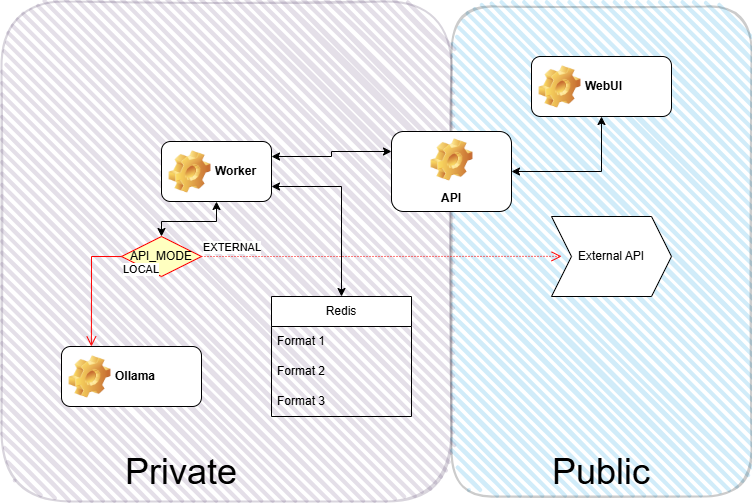
\includegraphics[width=1.0\textwidth]{src/architecture.png}
    \caption{High-level system architecture. Services are decomposed across public and private Docker networks, with the worker switching between LOCAL (Ollama) and EXTERNAL (OpenAI-compatible) inference depending on \texttt{API\_MODE}.}
    \label{fig:architecture_overview}
\end{figure}

\subsection{Service decomposition}

\textbf{WebUI (Streamlit).} Provides user-facing workflows: service health, log upload, format onboarding, report generation with progress tracking, and RAG-augmented chat.

\textbf{API gateway (FastAPI).} Exposes stable client endpoints and proxies requests to the worker. This layer isolates the client from internal worker changes.

\textbf{Worker (FastAPI).} Contains all domain logic: ingestion, format detection, normalisation, streaming metric computation, RAG indexing, agent execution, and report synthesis.

\textbf{Ollama.} Provides local model inference for both chat generation and embeddings. This supports privacy-preserving deployment without external telemetry sharing.

\textbf{Redis.} Stores approved format configurations, metric configurations per format, and historical baselines for trend analysis. Persistence is enabled to ensure configurations survive restarts.

\subsection{High-level data flow}

The end-to-end data flow proceeds from the user's browser through the Streamlit WebUI to the API gateway, which proxies requests to the internal worker service. The worker normalises uploaded logs, computes deterministic metrics, retrieves relevant regulatory context from the FAISS index, invokes the LLM and agent pipeline, renders the final Markdown report via Jinja2 templates, and writes the output to the shared \texttt{/out} volume. Redis persists approved configurations and historical baselines across sessions, while Ollama provides both chat completions and embedding generation. Figure~\ref{fig:pipeline_flow} illustrates the core processing pipeline in detail.

\begin{figure}[h]
    \centering
    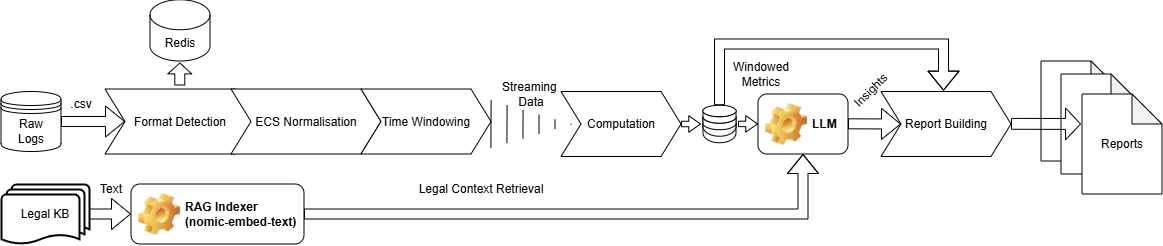
\includegraphics[width=1.0\textwidth]{src/data_flow.png}
    \caption{Core processing pipeline showing the deterministic ETL flow followed by grounded generation.}
    \label{fig:pipeline_flow}
\end{figure}

\section{Core Processing Pipeline}
\label{sec:core_pipeline}

The system's central component is the worker-side pipeline: \texttt{pipeline.py}. It implements a deterministic ETL-style flow followed by grounded generation.

\subsection{Log ingestion and format detection}
To support heterogeneous telemetry, ingestion begins with a \textit{format sniffer} that prioritises known formats in a fixed order (e.g.\ RBA header checks before generic CSV heuristics). The design supports two operational modes:

\textbf{Forced format mode.} A developer or operator can force a format via environment variables for controlled evaluations.

\textbf{Auto-detect mode.} The sniffer selects a format based on detection confidence and falls back to an \texttt{unknown} category.

\subsection{Normalisation to an ECS-inspired schema}
All records are mapped to a minimal, ECS-inspired event schema~\cite{ElasticECS}. A common schema simplifies downstream metric logic, enables consistent RAG context construction, and supports later expansion to additional log sources.

The normalisation layer produces canonical fields such as:
\texttt{@ts}, \texttt{user}, \texttt{src\_ip}, \texttt{dst\_ip}, \texttt{action}, \texttt{status}, \texttt{resource}, \texttt{msg}, and \texttt{raw}.

\subsection{Streaming metric computation}
Given the scale of authentication datasets (tens of millions of rows), the system uses a streaming accumulator rather than in-memory batch processing. Each record is processed once, updating counters and sets for:

\begin{itemize}
  \item total events,
  \item distinct users and IPs,
  \item authentication successes and failures,
  \item failure rate and repeated-failure IPs,
  \item attack-IP and takeover indicators.
\end{itemize}

This architecture maintains a near-constant memory footprint and supports realistic “production-like” datasets.

\subsection{Time-windowed reporting}
To produce audit-friendly outputs, metrics are grouped into configurable time windows (default: weekly or 90-day windows depending on deployment settings). Invalid timestamps are assigned to a special \textit{Unknown period} bucket, ensuring robust operation even with malformed data.

\section{RAG and Agent Subsystem Design}
\label{sec:rag_agent_design}

The RAG subsystem consists of two pipelines: an offline ingestion pipeline that indexes the regulatory knowledge base, and an online generation pipeline that retrieves relevant context at inference time. Figure~\ref{fig:rag_subsystem} illustrates both pipelines.

\begin{figure}[h]
    \centering
    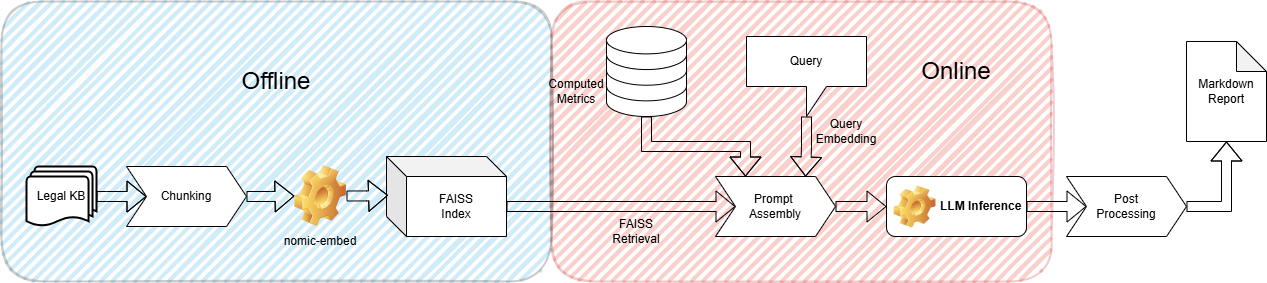
\includegraphics[width=1.0\textwidth]{src/RAG.png}
    \caption{RAG subsystem: an offline ingestion pipeline that chunks the regulatory knowledge base and builds a FAISS index using Nomic embeddings, and an online generation pipeline that retrieves relevant context at inference time and assembles the prompt for the LLM.}
    \label{fig:rag_subsystem}
\end{figure}

\subsection{Knowledge base ingestion and indexing}
The system maintains a knowledge base directory containing regulatory text split into smaller markdown units (e.g.\ per NIS2 article). These files are chunked and embedded using Nomic Embed~\cite{Nussbaum2024NomicEmbed} to build a FAISS vector index.

\subsection{FAISS-based retrieval}
Retrieval uses FAISS inner-product indices, enabling cosine similarity when embeddings are normalised. Retrieved chunks are appended to the LLM context, providing traceable grounding for compliance narratives.

The index includes both:
\begin{itemize}
  \item regulatory KB sources (NIS2 articles, ISO control summaries), and
  \item locally generated reports (for continuity and internal precedent).
\end{itemize}

\subsection{Confidence scoring for chat}
The chat subsystem computes a confidence score based on: index health, similarity of best match, source coverage, and context utilisation. This score is surfaced in the WebUI to convey uncertainty and to encourage verification when grounding is weak.

\subsection{Human-in-the-loop agents}
The system implements three agents that output structured JSON which must be approved before affecting the pipeline. Figure~\ref{fig:agent_workflow} illustrates the approval workflow.

\begin{figure}[h]
    \centering
    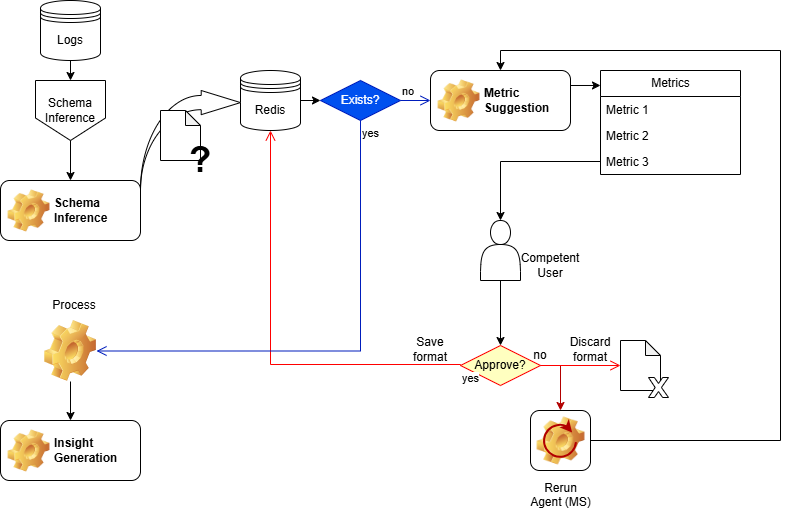
\includegraphics[width=1.0\textwidth]{src/agents.png}
    \caption{Human-in-the-loop agent approval workflow.}
    \label{fig:agent_workflow}
\end{figure}

\textbf{Schema inference agent.} Proposes ECS field mappings for new log formats.

\textbf{Metric suggestion agent.} Suggests additional metrics that are feasible given available fields and compliance goals.

\textbf{Insight generation agent.} Produces severity-tagged findings, evidence statements, and recommended controls. It also contains deterministic fallbacks (e.g.\ high failure rate thresholds) to avoid purely generative reasoning.

Approved schemas and metric definitions are stored in Redis to formalise onboarding decisions and support repeatable runs.

\section{Deployment, Security, and Hardware/Software Requirements}
\label{sec:deployment}

\subsection{Deployment model}
The system is deployed via Docker Compose to ensure reproducibility across environments. The design uses separate public/private networks and mounts shared volumes for \texttt{/data}, \texttt{/kb}, \texttt{/index}, and \texttt{/out}.

\subsection{Configuration management}
Runtime configuration is controlled via \texttt{.env}, with explicit switching between:

\textbf{LOCAL mode:} Ollama-backed inference and embeddings (privacy-preserving).

\textbf{EXTERNAL mode:} OpenAI-compatible inference endpoints for benchmarking (used only when policy permits).

\subsection{Hardware requirements}
Two deployment profiles are supported:

\textbf{CPU-only profile.} Sufficient for streaming metric computation, indexing on smaller KBs, and lightweight model inference.

\textbf{GPU-accelerated profile.} Recommended for acceptable latency when running modern local LLMs and large embedding workloads.

\subsection{Software stack}
The stack is implemented in Python microservices (FastAPI worker + gateway, Streamlit UI). The worker additionally uses FAISS for similarity search, Redis for persistence, and Jinja2 for report templating. All components are containerised and version-pinned through service requirements files.

\section{Summary}
\label{sec:system_design_summary}
The final design is a scalable, modular compliance reporting system combining deterministic log analytics with retrieval-grounded generative narration. It is explicitly engineered to support audit workflows by (i) normalising evidence into a consistent schema, (ii) computing metrics deterministically at scale, (iii) grounding generation in a retrieval layer, and (iv) requiring human approval for schema and metric onboarding.
%%%%%%%%


\chapter{Evaluation Methodology}
\label{chp:eval_methods}

This chapter describes the methodology used to evaluate the quality, reliability, and efficiency of the system's LLM-generated compliance reports. Because the system supports both local models (via Ollama) and external API-based models, a central research question is whether a lightweight, privacy-preserving local LLM can produce compliance documentation of comparable quality to larger cloud-hosted models. The evaluation framework is designed to answer this question using reproducible, automated metrics supplemented by statistical testing.

\section{Preliminary Experiment: LoRA Fine-Tuning vs.\ RAG}
\label{sec:lora_experiment_eval}

As noted in Section~\ref{sec:generation_strategy}, a preliminary experiment was conducted before the main evaluation to determine whether parameter-efficient fine-tuning could serve as a viable alternative to the RAG-based approach. This section presents the full experimental details and analysis.

\subsection{Experimental Setup}

The base model selected was \textbf{Qwen2.5-1.5B-Instruct}, chosen because its 1.5~billion parameters fit within the memory constraints of the available consumer-grade GPU (NVIDIA RTX 3050~Ti (4\,GB VRAM), CUDA~12.4) when loaded in 4-bit quantisation via BitsAndBytes (\texttt{nf4}, double quantisation, \texttt{float16} compute). A custom dataset of 25 instruction--response pairs was constructed from the NIS2 knowledge base, covering article summarisation, obligation extraction, and control-mapping tasks. Training was performed with the following LoRA configuration:

\begin{itemize}
    \item \textbf{Rank:} $r = 8$, \textbf{Alpha:} $\alpha = 16$, \textbf{Dropout:} 0.05
    \item \textbf{Target modules:} \texttt{q\_proj}, \texttt{k\_proj}, \texttt{v\_proj}, \texttt{o\_proj}
    \item \textbf{Trainable parameters:} 2,179,072 out of 1,545,893,376 (0.14\%)
    \item \textbf{Epochs:} 3, \textbf{Batch size:} 1 (gradient accumulation steps: 8)
    \item \textbf{Maximum sequence length:} 128 tokens
    \item \textbf{Optimiser:} \texttt{paged\_adamw\_8bit}
\end{itemize}

Training completed in approximately 39 seconds (12 steps), reaching a final training loss of 2.38.

\subsection{Results and Observed Failures}

The fine-tuned model was evaluated on the prompt \textit{``Summarize Article 21 of NIS2.''} Two representative outputs are shown below. In both cases, the model failed to produce an accurate summary of Article 21, instead generating hallucinated content that conflates NIS2 with GDPR-like provisions and invents obligations not present in the directive:

\textbf{Output 1} attributed obligations concerning ``security and privacy of personal data'' to Article 21, including requirements for cloud service providers, international data transfers, data anonymisation, and retention periods. None of these provisions appear in Article 21 of NIS2, which addresses \textit{cybersecurity risk-management measures}, not personal data processing.

\textbf{Output 2} was marginally more relevant, correctly identifying themes of incident response and risk assessment. However, it fabricated specific requirements (e.g., ``independent third-party risk assessments'', ``six-month activity log retention'') that do not appear in the directive text. It also incorrectly referred to the regulation as the ``Network and Information Systems Directive'' rather than the ``Network and Information Security Directive 2.''

\subsection{Analysis of Failure Factors}

Several compounding factors explain the poor quality of the fine-tuned outputs:

\begin{enumerate}
    \item \textbf{Insufficient training data.} The dataset contained only 25 examples, far below the hundreds or thousands typically required for LoRA fine-tuning to meaningfully shift model behaviour on a specialised domain.
    \item \textbf{Severe context truncation.} The maximum sequence length of 128 tokens meant that most training examples were truncated mid-sentence, preventing the model from learning complete regulatory reasoning chains or full article structures.
    \item \textbf{Hardware-imposed constraints.} The consumer-grade GPU necessitated 4-bit quantisation and a batch size of 1, limiting both model precision and effective gradient quality. These constraints, while necessary to fit the model in memory, reduced the capacity for domain adaptation.
    \item \textbf{No grounding mechanism.} Without retrieval augmentation, the model relied entirely on its pre-training knowledge and the minimal fine-tuning signal. When prompted about specific regulatory content, it defaulted to plausible-sounding but factually incorrect generalisations, a well-documented hallucination pattern in LLMs.
\end{enumerate}

\subsection{Implications for the Main Evaluation}

This experiment established two important baselines for the main evaluation. First, it confirmed that ungrounded generation, even with domain-specific fine-tuning, produces unacceptable hallucination rates for compliance documentation, validating the RAG-based architecture adopted in Chapter~\ref{chp:system_design}. Second, it demonstrated that effective LoRA fine-tuning for this domain would require substantially larger datasets, longer context windows ($\geq$1024 tokens), and more capable hardware. These findings motivate the focus of the remaining evaluation on comparing RAG-grounded generation across different LLM providers rather than comparing generation strategies.

\section{Evaluation Design Rationale}
\label{sec:eval_design_rationale}

A key architectural property of the system (Chapter~\ref{chp:system_design}) is that the report generation pipeline separates \textit{deterministic computation} from \textit{generative narration}. Specifically:

\begin{enumerate}
    \item \textbf{Metrics computation} is fully deterministic: the streaming accumulator computes identical metrics (failure rates, MFA coverage, attack indicators, etc.) regardless of which LLM is used.
    \item \textbf{Compliance observations} are generated by the first LLM call, which produces free-text prose summarising the metrics against regulatory requirements.
    \item \textbf{AI-generated insights} are produced by the Insight Generation Agent via a second LLM call, which returns structured JSON containing severity-tagged findings, evidence linkage, trend analysis, and recommendations.
\end{enumerate}

This separation enables a controlled comparison: the same input metrics are presented to different LLM providers, and only the generative outputs (steps 2 and 3) vary. The evaluation therefore focuses exclusively on the quality and characteristics of these LLM-produced sections.

\section{Pipeline Instrumentation}
\label{sec:instrumentation}

To capture the data needed for evaluation, the report generation pipeline (\texttt{pipeline.py}) and the Insight Generation Agent (\texttt{insight\_agent.py}) were instrumented with structured logging. Each pipeline execution produces a JSON log entry containing:

\begin{itemize}
    \item \textbf{Identifiers:} unique run ID, ISO-8601 timestamp, provider mode (\texttt{LOCAL} or \texttt{EXTERNAL}), model name, time period, and compliance framework.
    \item \textbf{Input snapshot:} the complete metrics dictionary passed to both LLM calls, enabling post-hoc verification of factual claims.
    \item \textbf{Compliance call data:} wall-clock latency, prompt and response lengths (characters and estimated tokens), raw LLM response text, and success/error status.
    \item \textbf{Insight call data:} the same timing and length fields as the compliance call, plus:
    \begin{itemize}
        \item whether JSON could be extracted from the response (regex extraction success),
        \item whether the extracted JSON was syntactically valid (\texttt{json.loads} success),
        \item the raw parsed JSON before the system's validation and normalisation layer modifies it,
        \item the number of findings generated by the LLM versus the number added by deterministic heuristic fallbacks,
        \item a full schema validation report (described in Section~\ref{sec:schema_conformance}).
    \end{itemize}
    \item \textbf{Pipeline totals:} end-to-end wall-clock time and final rendered report length in characters.
\end{itemize}

All instrumentation is wrapped in exception handlers to ensure that logging failures never interrupt normal pipeline operation. Log entries are appended to a JSONL (JSON Lines) file, where each line represents one complete pipeline run.

\section{Automated Evaluation Metrics}
\label{sec:eval_metrics}

The evaluation framework defines nine fully automated metrics, organised into three categories: \textit{structural compliance}, \textit{analytical quality}, and \textit{operational performance}. All metrics are computed by a dedicated Jupyter analysis notebook (\texttt{notebooks/llm\_evaluation.ipynb}) that reads the JSONL evaluation log produced by the instrumented pipeline (Section~\ref{sec:instrumentation}), flattens each run into a tabular representation using \texttt{pandas}, and produces the summary tables and figures presented in Chapter~\ref{chp:eval_results}. The notebook depends only on \texttt{pandas}, \texttt{numpy}, \texttt{matplotlib}, \texttt{seaborn}, and \texttt{scipy}, which keeps the evaluation reproducible from a single log file without introducing additional tooling to the project.

\subsection{Structural Compliance Metrics}

These metrics measure whether the LLM can follow the system's output format instructions, which is a prerequisite for the generated insights to be used in the report pipeline.

\subsubsection{JSON Parse Success Rate}
\label{sec:json_parse}

The Insight Generation Agent instructs the LLM to return a JSON object matching a specified schema. This metric measures:

\begin{itemize}
    \item \textbf{JSON extraction rate:} the percentage of responses from which any JSON object could be extracted via regex.
    \item \textbf{JSON parse rate:} the percentage of extracted JSON strings that are syntactically valid (i.e.\ pass \texttt{json.loads} without error).
\end{itemize}

If the LLM fails to produce valid JSON, the system falls back to an error response, and the entire insight section of the report is replaced with heuristic-only content. A low JSON parse rate therefore indicates fundamental instruction-following failure.

\subsubsection{Schema Conformance Rate}
\label{sec:schema_conformance}

Even when JSON parses successfully, it may not conform to the expected structure. The schema validation checks three levels:

\begin{enumerate}
    \item \textbf{Top-level key presence:} whether the JSON contains all five required keys: \texttt{summary}, \texttt{risk\_level}, \texttt{findings}, \texttt{positive\_observations}, and \texttt{trend\_analysis}. Reported as a percentage of expected keys present.
    \item \textbf{Risk level validity:} whether the \texttt{risk\_level} value is a member of the valid enum \{low, medium, high, critical\}.
    \item \textbf{Overall conformance:} a composite score averaging top-level key presence, risk level validity, and mean finding-level field completeness.
\end{enumerate}

\subsubsection{Finding Field Completeness}

For each finding in the \texttt{findings} array, the validator checks for the presence of nine expected fields: \texttt{id}, \texttt{severity}, \texttt{category}, \texttt{title}, \texttt{description}, \texttt{evidence}, \texttt{compliance\_impact}, \texttt{recommendation}, and \texttt{priority}. Completeness is reported as a ratio per finding and aggregated as a mean across all findings per run.

Missing fields are assigned default values by the system's validation layer (\texttt{\_validate\_finding}), so this metric captures how much of the response structure the LLM generated autonomously versus how much was filled in by the system.

\subsubsection{Severity Distribution Validity}

Each finding's \texttt{severity} value is checked against the valid enum \{critical, high, medium, low, info\}. This metric reports the percentage of LLM-generated severity values that are valid members without requiring normalisation.

\subsection{Analytical Quality Metrics}

These metrics measure the depth and independence of the LLM's analytical output.

\subsubsection{Findings Origin: LLM vs.\ Heuristic}

The Insight Generation Agent contains deterministic fallback heuristics that inject findings for common patterns (e.g.\ authentication failure rate exceeding 25\%, MFA coverage below 100\%). These heuristics fire after the LLM's findings to ensure minimum coverage.

This metric tracks:
\begin{itemize}
    \item the number of findings generated by the LLM (before heuristic enhancement),
    \item the number of findings added by heuristic rules,
    \item the total finding count in the final report.
\end{itemize}

A higher proportion of LLM-originated findings indicates stronger analytical capability, as the model is independently identifying the same issues that the heuristics would otherwise catch.

\subsubsection{Response Length Distribution}

Report length (in characters) and raw LLM response length are recorded per run. While length alone does not indicate quality, systematic differences between providers may indicate varying levels of detail, verbosity, or analytical depth. This metric is reported as box plots to visualise the distribution across runs.

\subsection{Operational Performance Metrics}

\subsubsection{Latency}

Wall-clock latency is recorded at three levels:
\begin{itemize}
    \item \textbf{Compliance call latency:} time for the first LLM call (free-text compliance observations).
    \item \textbf{Insight LLM call latency:} time for the second LLM call only (excluding parsing and heuristic post-processing).
    \item \textbf{Full pipeline latency:} end-to-end time from the start of \texttt{generate\_report()} to the final rendered Markdown output.
\end{itemize}

Latency is a critical operational metric for deployment feasibility: local models deployed on consumer hardware must achieve acceptable response times for interactive use.

\subsubsection{Token and Cost Estimation}

Token counts are estimated from character lengths using a $\div 4$ heuristic (a standard approximation for subword tokenisers). Per-run cost is computed using configurable rate tables (\$ per 1K tokens, input and output priced separately). For local models, cost is reported as zero (amortised hardware cost is excluded). This metric enables a direct cost--quality trade-off comparison between providers.

\subsubsection{Cross-Run Consistency}

For configurations where multiple runs are available for the same (provider, model, period) triple, consistency is measured using the \textit{coefficient of variation} (CV = $\sigma / \mu$) across:
\begin{itemize}
    \item total finding count,
    \item LLM-originated finding count,
    \item rendered report length.
\end{itemize}

A lower CV indicates more deterministic behaviour. This metric is particularly relevant for compliance contexts where reproducibility of reports is desirable.

\section{Experimental Setup}
\label{sec:experimental_setup}

\subsection{Models Under Comparison}

The evaluation compares outputs from three models:
\begin{itemize}
    \item \textbf{Local (Ollama):} \texttt{llama3.1:8b}, deployed via the Ollama service container with a 600-second timeout.
    \item \textbf{External API -- Qwen3-32B:} \texttt{Qwen/Qwen3-32B-TEE}, accessed via an OpenAI-compatible endpoint with a 120-second timeout and temperature fixed at 0.2 for reproducibility.
    \item \textbf{External API -- GPT-5.4-nano:} \texttt{gpt-5.4-nano}, accessed via the same endpoint configuration. The model is referred to throughout this report by the identifier exposed by the deployed endpoint; this string is the label returned by the provider's API and is used here as the canonical name for that configuration rather than as a claim about an externally published model release.
\end{itemize}

The local model represents the privacy-preserving deployment scenario, while the two external models serve as quality benchmarks at different capability tiers.

\subsection{Evaluation Dataset}

The system processes the RBA authentication dataset across multiple 90-day time windows. Each window produces a deterministic metrics dictionary that is then passed to all three LLM configurations. The evaluation was conducted across seven distinct 90-day windows (six dated windows plus one ``Unknown period'' bucket for records with missing timestamps), with five runs per window per model to support consistency analysis and statistical testing.

\subsection{Run Protocol}

For each (model, period) pair, the pipeline is executed multiple times to accumulate sufficient data for consistency analysis and statistical testing. The target is ideally a minimum of five runs per configuration per period to achieve reasonable statistical power for non-parametric tests.

\section{Statistical Testing}
\label{sec:statistical_testing}

When sufficient paired data is available, differences between providers are measured using:

\begin{itemize}
    \item \textbf{Mann--Whitney U test} (non-parametric, does not assume normality): tests whether the distributions of a given metric differ significantly between two providers. A significance threshold of $p < 0.05$ is used.
    \item \textbf{Cohen's $d$ effect size:} quantifies the practical magnitude of observed differences using pooled standard deviations. Effect sizes are classified as negligible ($|d| < 0.2$), small ($0.2 \leq |d| < 0.5$), medium ($0.5 \leq |d| < 0.8$), or large ($|d| \geq 0.8$).
\end{itemize}

Statistical tests are applied to key metrics including latency, schema conformance, finding count, and report length. Results are presented as comparison tables with $p$-values and effect sizes.

\section{Limitations of the Automated Evaluation}
\label{sec:eval_limitations}

The fully automated metrics described above measure structural, operational, and consistency properties of the LLM outputs. However, they do not directly measure several qualitative dimensions that are important for compliance documentation, including factual accuracy, hallucination rate, legal citation accuracy, and actionability of recommendations.

\section{LLM-as-a-Judge Evaluation for Regulatory Alignment}
\label{sec:llm_judge_methodology}
 
To address the qualitative gaps identified in Section~\ref{sec:eval_limitations}, a supplementary evaluation using the \textit{LLM-as-a-Judge} paradigm\cite{ZhengMTBench2023} is performed. This approach uses frontier LLMs as automated evaluators, scoring generated reports against structured rubrics. Recent work has demonstrated that LLM judges achieve over 80\% agreement with human evaluators\cite{ZhengMTBench2023}, and the approach has been successfully applied to legal and regulatory text evaluation\cite{LeMAJ2025}.
 
The judge evaluation is implemented directly in Python as an extension of the same notebook pipeline used for the automated metrics. Each generated report is read back from the evaluation log, wrapped in a scoring prompt together with its input metrics and the rubric for one evaluation dimension, and submitted to each judge model via its API. The judges' numeric responses are parsed, aggregated, and saved alongside the other CSV artefacts produced by the notebook. Keeping the judge evaluation inside the existing notebook avoids introducing a separate evaluation toolchain and ensures that every judge score is linked to a specific run in the main log by \texttt{run\_id}.
 
\subsection{Evaluation Dimensions and Rubric Design}
 
Each generated compliance report is evaluated on four dimensions using a 1--5 Likert scale with explicit score-level definitions:
 
\begin{enumerate}
    \item \textbf{Regulatory Accuracy} (1--5): Whether cited NIS2 articles, obligations, and requirements are factually correct and properly attributed. \textit{Score 1:} contains multiple factual errors about NIS2 or fabricates requirements; \textit{Score 5:} all cited articles and obligations are correct and properly attributed.
    \item \textbf{Completeness} (1--5): Whether the report covers the relevant NIS2 Article~21(2) requirements for the access-control scenario. The rubric anchors completeness to the subset of mandatory measures most relevant to access control specifically (a)~risk analysis policies, (b)~incident handling, (i)~human resources security and access control, and (j)~multi-factor authentication and continuous authentication, rather than the full ten-measure list, since several NIS2 measures (e.g.\ supply-chain security) are out of scope for an access-control report.
    \item \textbf{Faithfulness to Evidence} (1--5): Whether every claim in the report is grounded in either the computed metrics or the retrieved regulatory text. \textit{Score 1:} majority of claims are unsupported or fabricated; \textit{Score 5:} all claims are traceable to input data or retrieved context.
    \item \textbf{Actionability} (1--5): Whether recommendations are specific and implementable rather than vague or generic. \textit{Score 1:} recommendations are generic platitudes; \textit{Score 5:} recommendations reference specific controls, timelines, or technical measures.
\end{enumerate}
 
\subsection{Multi-Judge Panel Design}
 
To mitigate known biases in LLM-as-a-judge evaluation, including self-enhancement bias, where models favour their own outputs\cite{ZhengMTBench2023}, a panel of two diverse judge models from different vendors is used: Claude (Anthropic) and GPT (OpenAI). A third judge, Google's Gemini, was originally considered as part of the panel in line with the Panel of LLM Evaluators (PoLL) recommendation\cite{Verga2024PoLL} that diverse judge panels outperform any single judge, but was dropped after repeated API reliability issues during pilot runs made it impractical to obtain a complete set of scores for every (report, dimension) pair. The remaining two judges are still drawn from different vendors with different underlying model families, which preserves the core rationale of the PoLL approach, diversity of training data and alignment strategies, even if the panel is smaller than originally planned.
 
Concretely, the notebook iterates over the cross product of (report, judge, dimension). For each triple it constructs a prompt containing the rubric for that dimension, the report text, and the source model identifier, and asks the judge to return a single integer score and a one-sentence justification in a fixed JSON format. Temperature is set to zero on every judge call to maximise determinism, and responses are parsed defensively with a fallback regex in case the judge wraps its JSON in Markdown fences; any unparseable response is flagged for manual review rather than silently discarded. Scores are then pivoted into per-(source model, judge, dimension) tables and visualised as grouped bar charts comparing the three source models across the four dimensions.

Inter-judge agreement is reported using Cohen's~$\kappa$ with linear weighting, which is appropriate for ordinal scales because it penalises a one-step disagreement less than a four-step disagreement. To detect self-enhancement bias, a per-vendor comparison is performed: GPT's scores on GPT-generated reports are compared against Claude's scores on the same reports, and a delta of more than 0.3 points is flagged as evidence of bias. When a self-enhancement effect is detected, a \textit{bias-adjusted} aggregate score is computed for the affected source model by excluding the same-vendor judge's ratings; for source models without a corresponding self-vendor judge (LLaMA via Ollama, Qwen), both judges' scores are retained.

\subsection{Sampling Strategy}
\label{sec:judge_sampling}

A full panel evaluation over all 105 generated reports would require 840 API calls (105 reports $\times$ 4 dimensions $\times$ 2 judges) plus a further 105 for coverage scoring, taking on the order of 70 minutes of wall-clock time and incurring non-trivial cost. To keep the evaluation tractable while preserving statistical power, a stratified sub-sample of 12 reports per source model (36 reports overall) is drawn, balanced across the seven 90-day reporting windows so that every period is represented for every model. The reduced sample still yields 288 rubric scores, 36 reports per (judge, dimension) cell, which is more than adequate for the Mann--Whitney U comparisons reported in Chapter~\ref{chp:eval_results}.
 
\subsection{Access Control Topic Coverage}
\label{sec:access_control_coverage}
 
A binary coverage metric complements the Likert-scale evaluation by checking which sub-topics of access control the report substantively addresses. The original methodology proposed mapping reports against the ten NIS2 Article~21(2)(a)--(j) measures verbatim, but pilot runs showed that this checklist is largely uninformative for an access-control-only report: measures such as supply-chain security or business continuity are out of scope and consistently scored \texttt{false}, compressing every report into the same 2/10 region regardless of quality. A more discriminative checklist of twelve access-control sub-topics drawn from NIS2 Article~21(2)(i) and (j) and ISO/IEC~27001 control A.9 is therefore used: authentication failure analysis, MFA coverage, privileged access review, account lockout policies, password policy compliance, source IP reputation, session management, periodic access review cadence, role-based access control and least-privilege analysis, anomalous login behaviour detection, explicit regulatory mapping, and trend analysis across reporting windows. A single judge prompt presents the report and the twelve topics, and asks for a JSON response with a Boolean per topic plus an aggregate count; the coverage scoring uses one judge (Claude) rather than the full panel because the binary nature of the question yields lower judge variance and the cost of a panel was not justified by the additional information.
 
\subsection{Viability Assessment}
\label{sec:viability_assessment}
 
To address the project's objective of evaluating whether the system can reduce the manual effort required for compliance reporting, a time-comparison analysis contextualises the pipeline's generation speed against industry benchmarks for manual compliance documentation. The system's end-to-end generation time (mean full-pipeline latency ranging from 17.2~seconds for GPT-5.4-nano to 101.6~seconds for the local LLaMA, with worst-case runs reaching 178~seconds; see Section~\ref{sec:latency_results}) is compared against published estimates of manual compliance effort, providing a quantitative basis for assessing practical viability.

\chapter{Evaluation Results}
\label{chp:eval_results}
 
This chapter presents the evaluation results across the three metric categories defined in Chapter~\ref{chp:eval_methods}: structural compliance, analytical quality, and operational performance. All results are derived from a balanced set of 105 pipeline runs, exported by the evaluation notebook from the JSONL log. The comparison covers three model configurations: the local \texttt{llama3.1:8b} served via Ollama, and two external API models, \texttt{Qwen/Qwen3-32B-TEE} and \texttt{gpt-5.4-nano}, with 35~runs per model, spread across seven 90-day evaluation windows (five runs per window per model) to support both aggregate comparisons and the cross-run consistency analysis.
 
\section{Structural Compliance Metrics}
\label{sec:results_structural}
 
\subsection{JSON Parse Success Rate}
 
\begin{figure}[h]
    \centering
    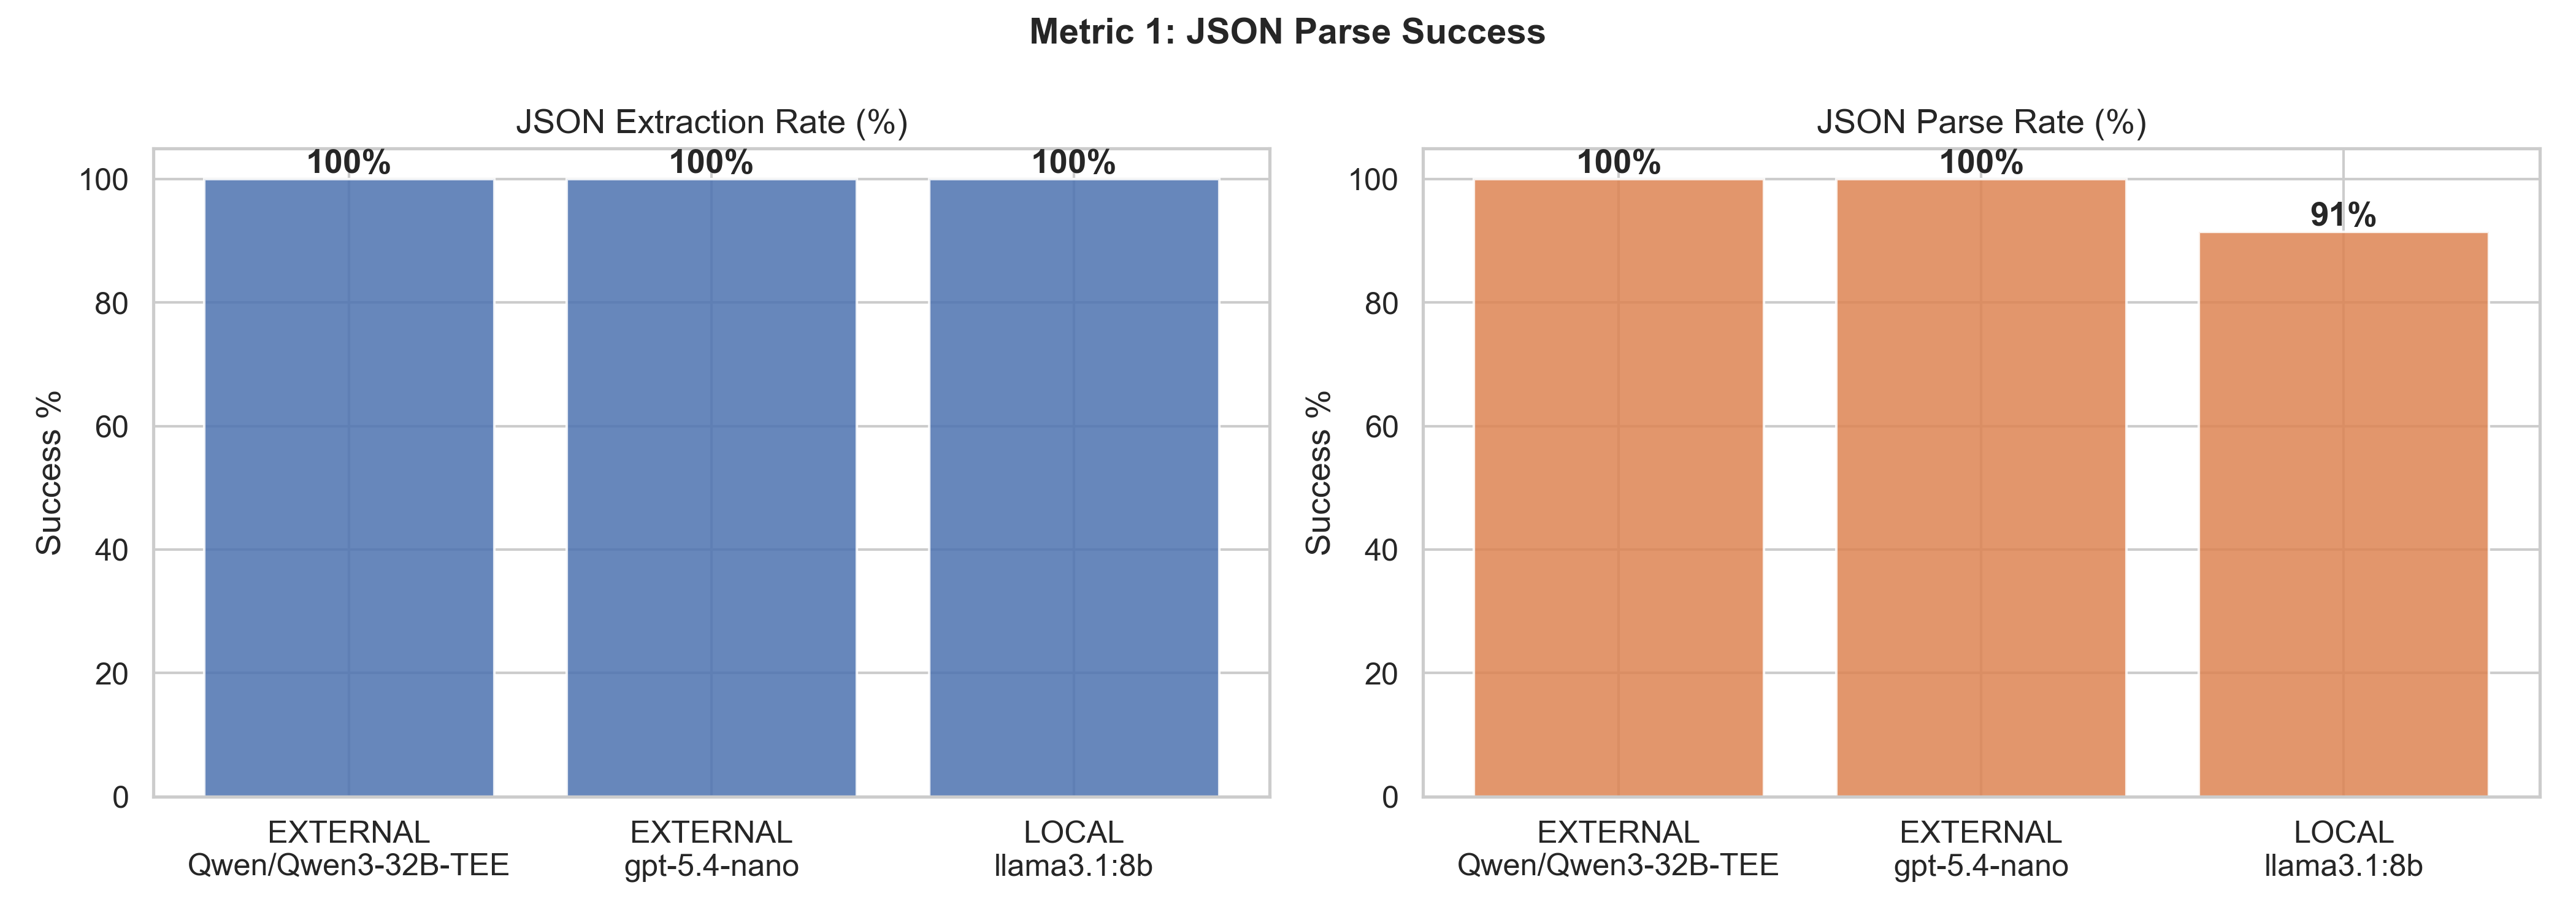
\includegraphics[width=1.0\textwidth]{src/json_parse_success_rates.png}
    \caption{JSON extraction and parse success rates across providers.}
    \label{fig:json_parse_success}
\end{figure}
 
Both external models returned a syntactically valid JSON object on every single run, giving a 100\% JSON parse rate across all 35 runs each. The local LLaMA model succeeded on 32 of its 35 runs (91.4\%); in the three failing runs, the raw response contained malformed JSON that could not be recovered by the extraction regex and caused \texttt{json.loads} to raise. The pipeline's heuristic fallback ensured that a report was still produced in those cases, but the insight section relied entirely on deterministic rules rather than LLM analysis. For production use this gap remains non-trivial: roughly one in twelve local-model runs still requires a retry or degrades to a rule-based report, even though the rate has improved on the larger dataset.
 
\subsection{Schema Conformance Rate}
 
\begin{figure}[h]
    \centering
    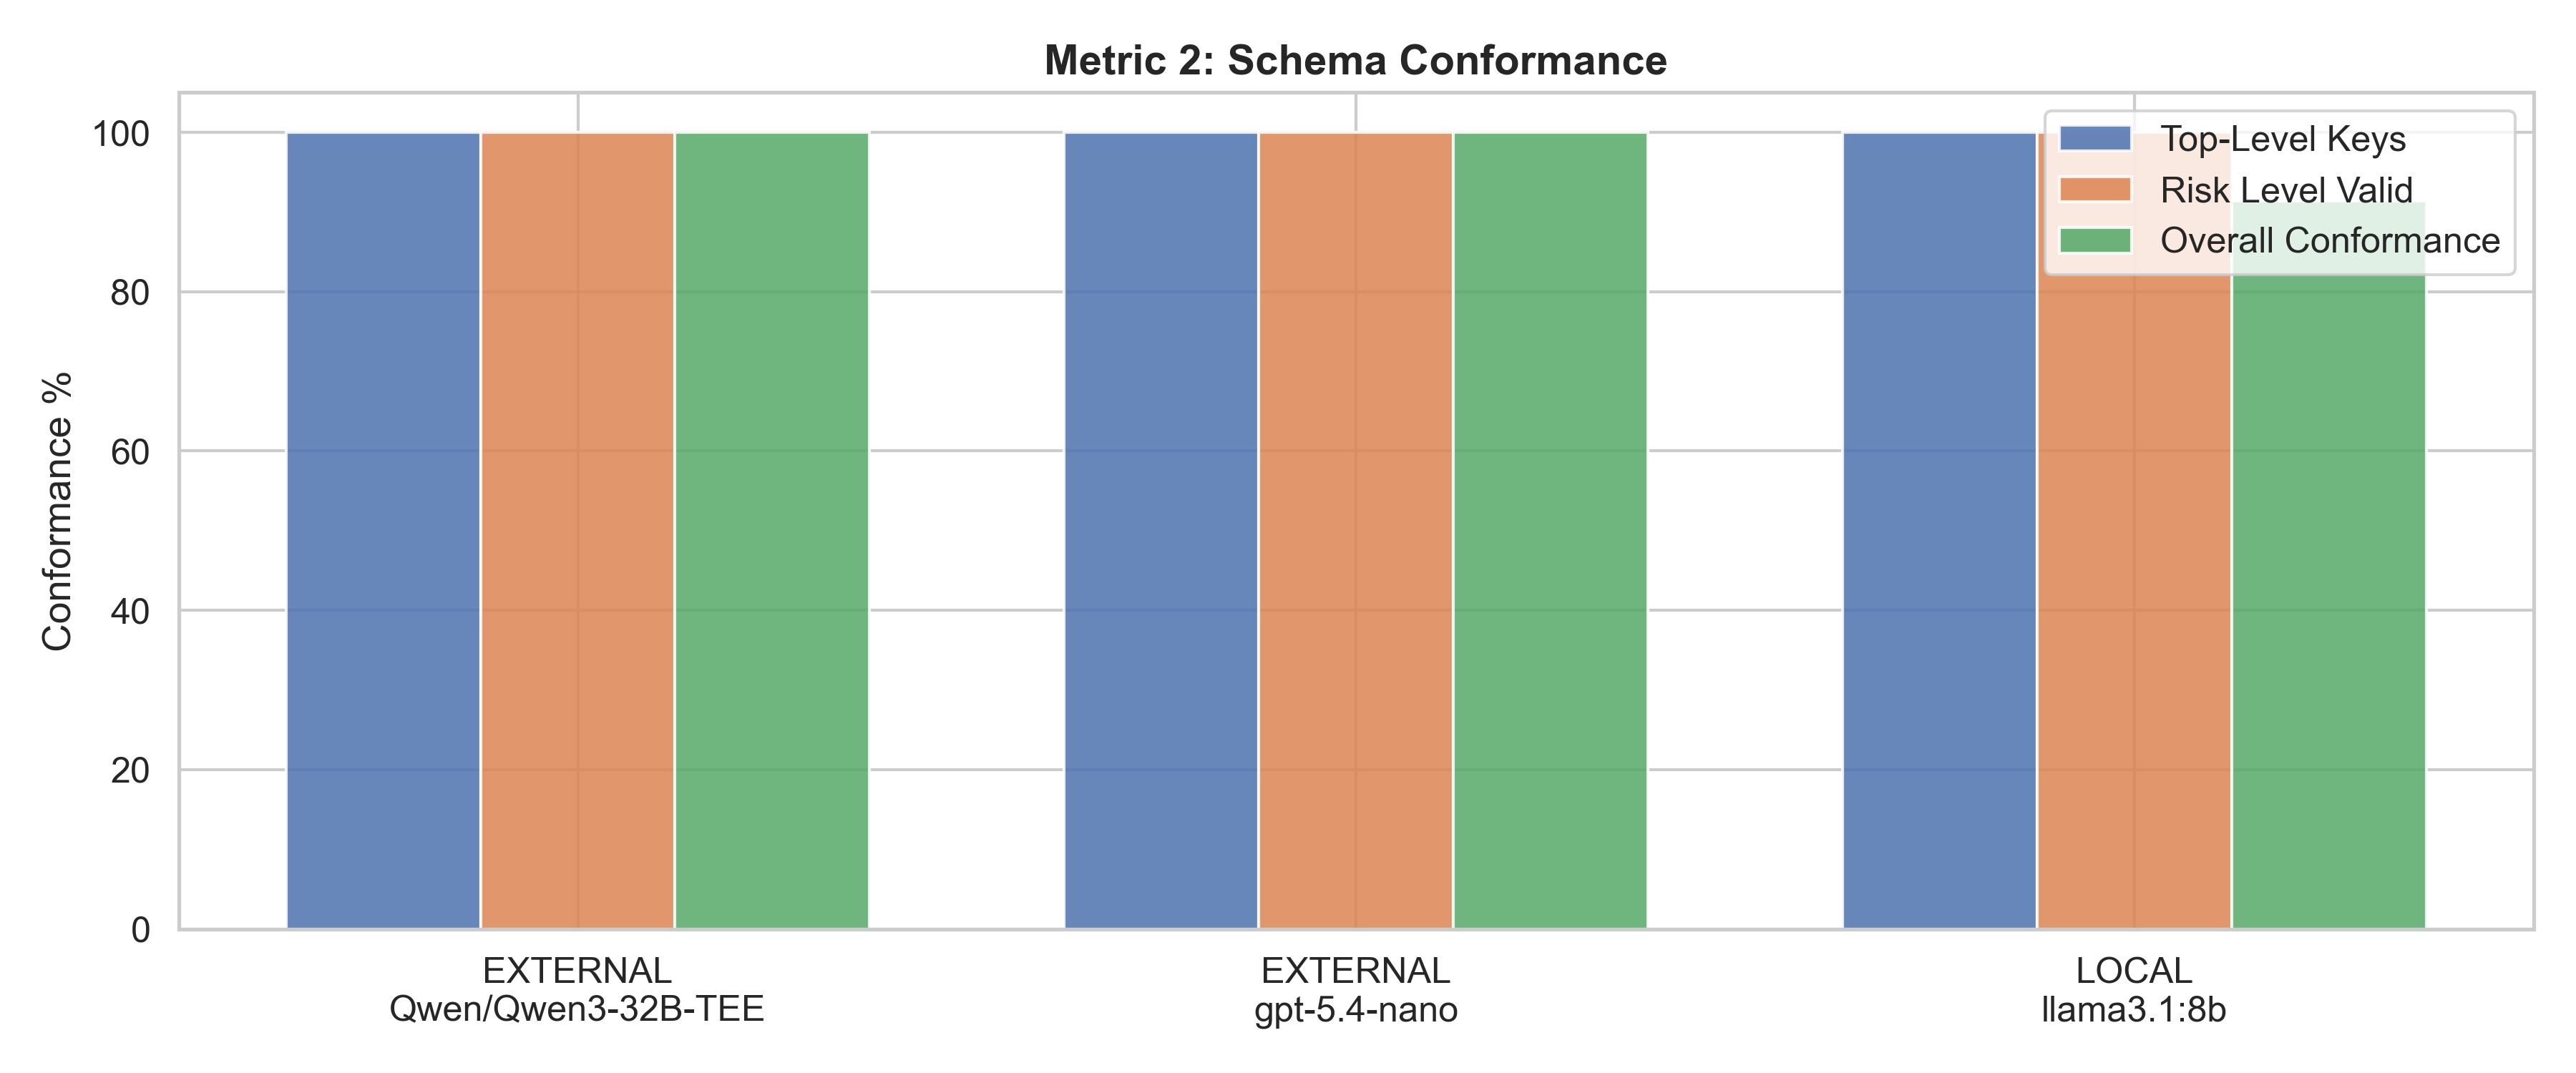
\includegraphics[width=1.0\textwidth]{src/schema_conformance_rates.png}
    \caption{Schema conformance broken down by top-level key presence, risk-level enum validity, and overall conformance.}
    \label{fig:schema_conformance}
\end{figure}
 
\begin{table}[!ht]
    \centering
    {\footnotesize
        \begin{tabular}{|l|l|r|r|r|r|}
        \hline
            \textbf{Provider} & \textbf{Model} & \textbf{Runs} & \textbf{Top-level (\%)} & \textbf{Risk level valid (\%)} & \textbf{Overall (\%)} \\ \hline
            EXTERNAL & Qwen/Qwen3-32B-TEE & 35 & 100.0 & 100.0 & 100.0 \\ \hline
            EXTERNAL & gpt-5.4-nano       & 35 & 100.0 & 100.0 & 100.0 \\ \hline
            LOCAL    & llama3.1:8b        & 35 & 100.0 & 100.0 &  91.4 \\ \hline
        \end{tabular}
    }
    \caption{Schema conformance by provider and model.}
    \label{tab:schema_conformance}
\end{table}
 
Schema conformance tells a consistent story. Every response that parsed as JSON also contained all five required top-level keys (\texttt{summary}, \texttt{risk\_level}, \texttt{findings}, \texttt{positive\_observations}, \texttt{trend\_analysis}) and a valid \texttt{risk\_level} enum value. The overall conformance figure for the local model (91.4\%) therefore tracks its JSON parse rate exactly: the three failures were catastrophic rather than partial. In short, once the local model produces JSON at all, it adheres to the schema; the risk is on the outer envelope, not on the internal structure.
 
\subsection{Finding Field Completeness}
 
\begin{figure}[h]
    \centering
    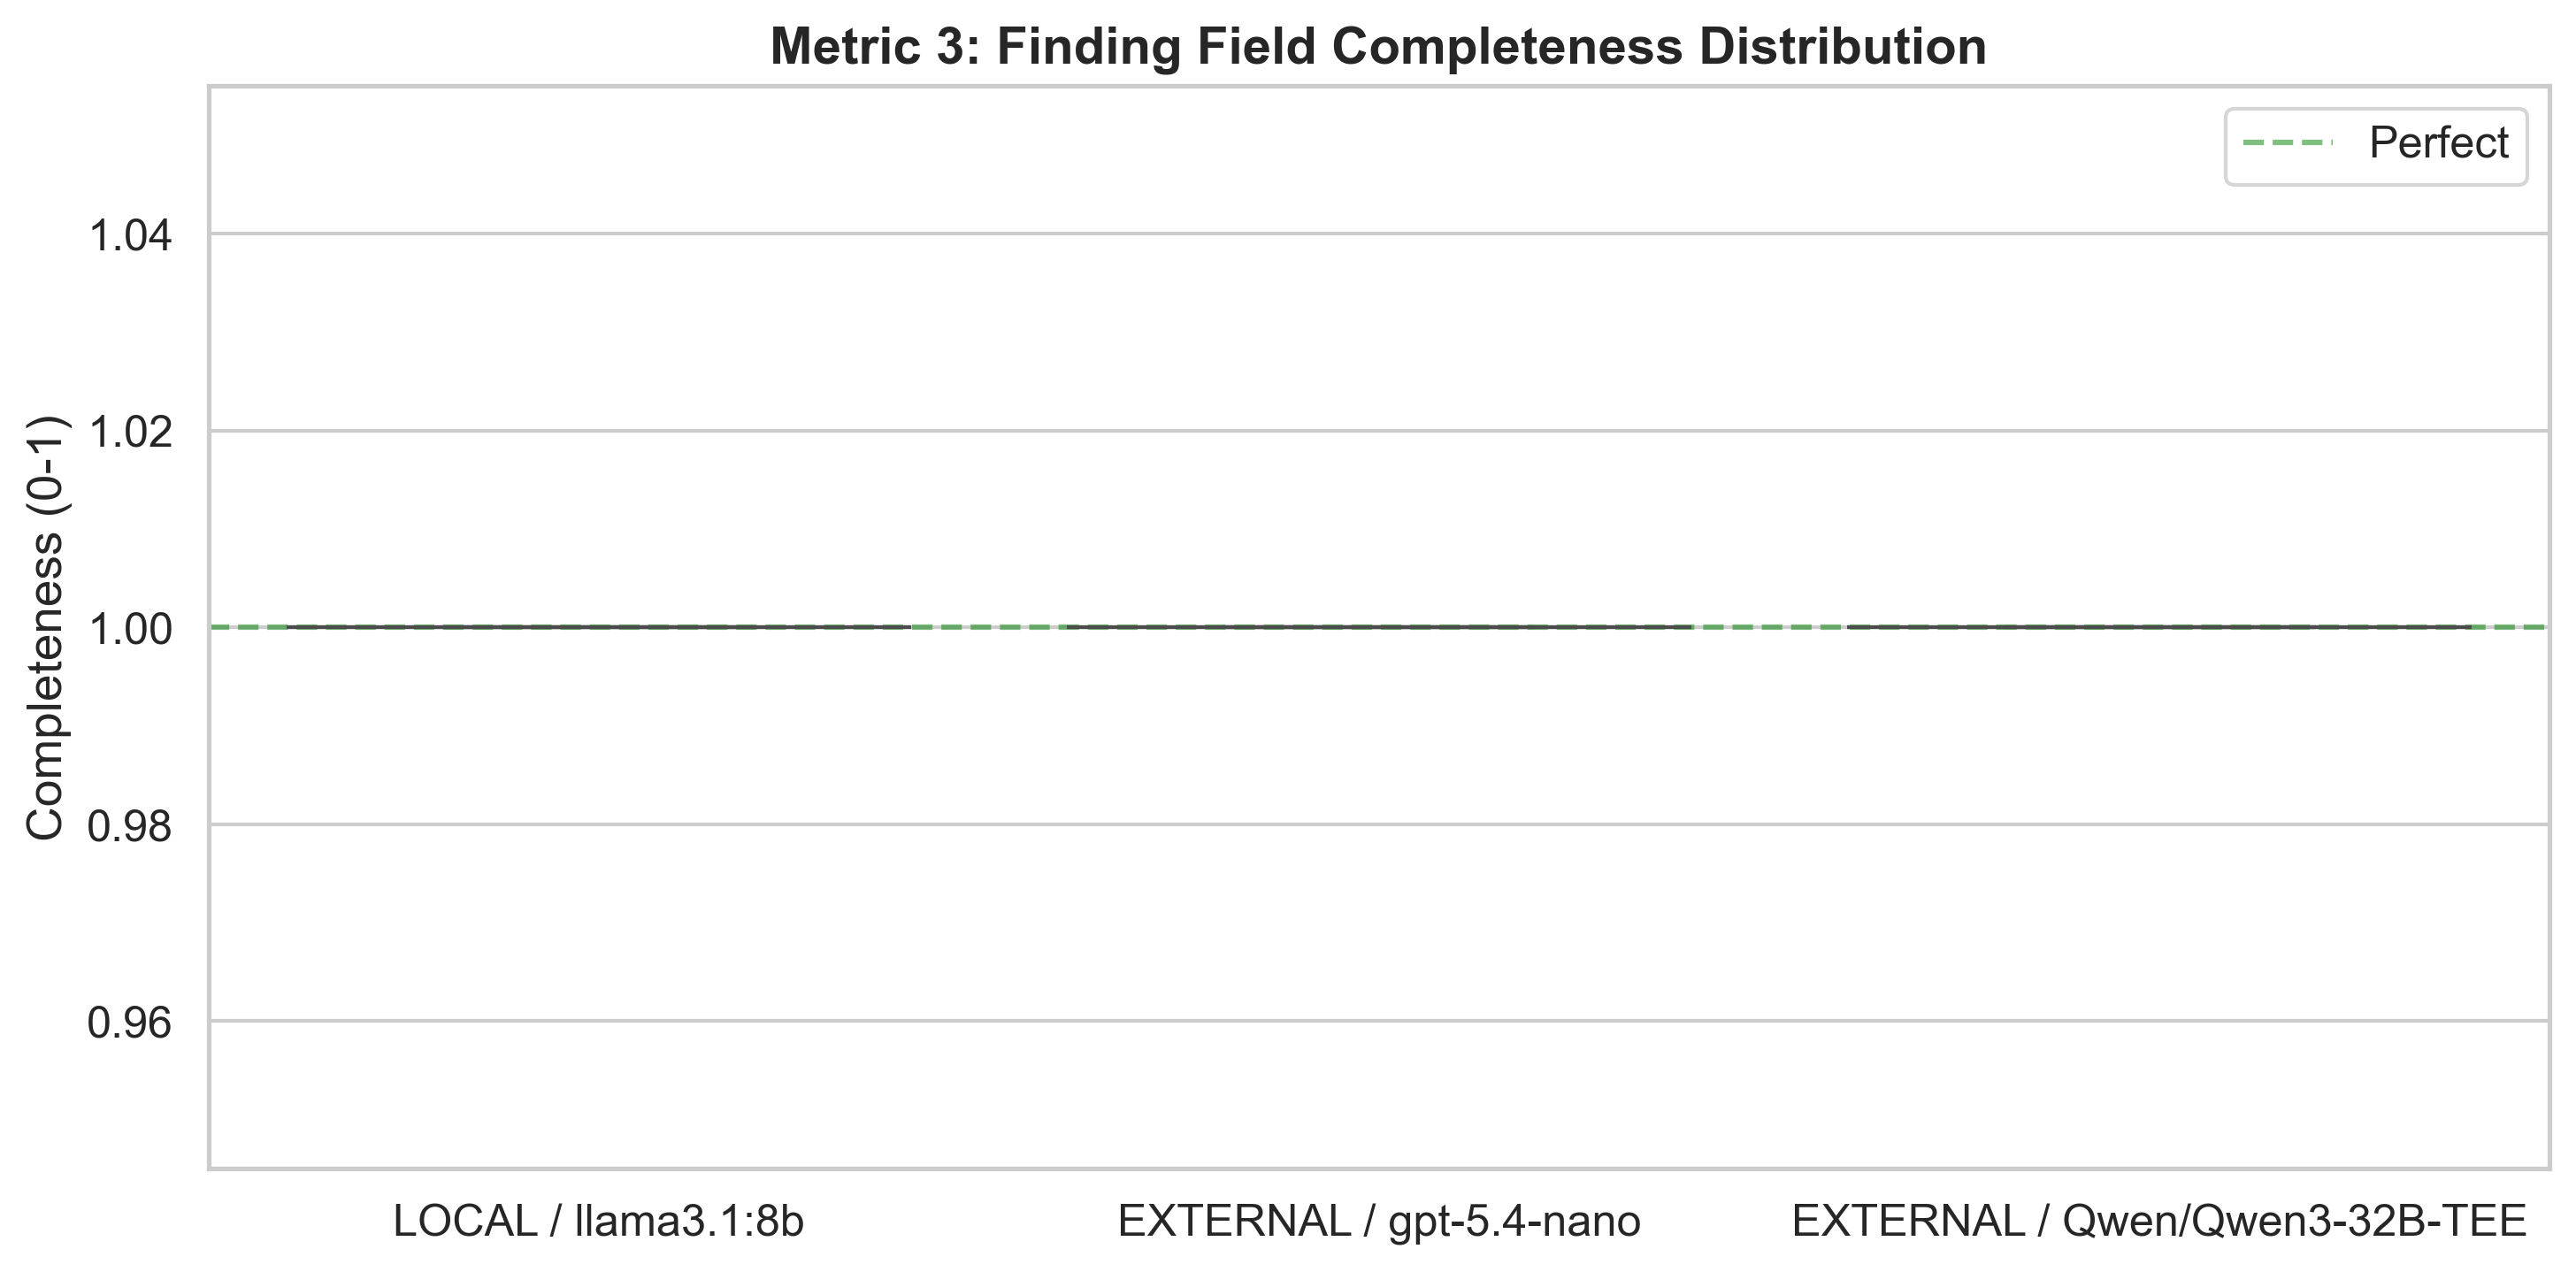
\includegraphics[width=1.0\textwidth]{src/finding_completeness.png}
    \caption{Distribution of finding field completeness. All three models produce fully populated findings across every run.}
    \label{fig:finding_completeness}
\end{figure}
 
\begin{table}[!ht]
    \centering
    {\footnotesize
        \begin{tabular}{|l|l|r|r|r|r|}
        \hline
            \textbf{Provider} & \textbf{Model} & \textbf{Findings} & \textbf{Mean} & \textbf{Median} & \textbf{Fully complete (\%)} \\ \hline
            EXTERNAL & Qwen/Qwen3-32B-TEE & 105 & 1.00 & 1.00 & 100.0 \\ \hline
            EXTERNAL & gpt-5.4-nano       & 149 & 1.00 & 1.00 & 100.0 \\ \hline
            LOCAL    & llama3.1:8b        &  95 & 1.00 & 1.00 & 100.0 \\ \hline
        \end{tabular}
    }
    \caption{Finding field completeness aggregated across all LLM-originated findings.}
    \label{tab:finding_completeness}
\end{table}
 
For each LLM-originated finding that actually reached the report, all nine expected fields (\texttt{id}, \texttt{severity}, \texttt{category}, \texttt{title}, \texttt{description}, \texttt{evidence}, \texttt{compliance\_impact}, \texttt{recommendation}, \texttt{priority}) were present in every case, across all 349 findings produced by the three models combined. This is a strong instruction-following result and indicates that the system's validation layer rarely needs to fill in default values when the LLM succeeds at producing a finding at all. The field-level completeness metric and the JSON-level parse metric thus capture complementary failure modes: the latter measures whether the envelope is syntactically correct, the former measures whether the internal items are populated.
 
\subsection{Severity Distribution Validity}
 
\begin{table}[!ht]
    \centering
    {\footnotesize
        \begin{tabular}{|l|l|r|r|r|r|r|}
        \hline
            \textbf{Provider} & \textbf{Model} & \textbf{critical} & \textbf{high} & \textbf{medium} & \textbf{low} & \textbf{info} \\ \hline
            EXTERNAL & Qwen/Qwen3-32B-TEE & 40 & 50 & 15 & 0 & 0 \\ \hline
            EXTERNAL & gpt-5.4-nano       & 60 & 57 & 31 & 1 & 0 \\ \hline
            LOCAL    & llama3.1:8b        & 27 & 33 & 30 & 5 & 0 \\ \hline
        \end{tabular}
    }
    \caption{Distribution of severity labels assigned across all LLM-generated findings.}
    \label{tab:severity_distribution}
\end{table}
 
\begin{table}[!ht]
    \centering
    {\footnotesize
        \begin{tabular}{|l|l|r|r|r|}
        \hline
            \textbf{Provider} & \textbf{Model} & \textbf{Findings} & \textbf{Valid} & \textbf{Validity (\%)} \\ \hline
            EXTERNAL & Qwen/Qwen3-32B-TEE & 105 & 105 & 100.0 \\ \hline
            EXTERNAL & gpt-5.4-nano       & 149 & 149 & 100.0 \\ \hline
            LOCAL    & llama3.1:8b        &  95 &  95 & 100.0 \\ \hline
        \end{tabular}
    }
    \caption{Severity enum validity by provider and model.}
    \label{tab:severity_validity}
\end{table}
 
All three models produced severity labels drawn exclusively from the valid enum \{critical, high, medium, low, info\}, so the strict validity rate is 100\% across the board. The distributions (Table~\ref{tab:severity_distribution}) are more interesting: the external models skew towards the \texttt{critical} and \texttt{high} end of the scale, while the local model distributes findings more evenly, giving a noticeably higher share to \texttt{medium} and \texttt{low}. None of the three models emitted any \texttt{info}-level findings in this dataset. Whether the external models' higher-severity bias reflects sharper judgement or a prompt-following tendency to overstate risk would require the LLM-as-a-Judge evaluation (Section~\ref{sec:llm_judge_methodology}) to answer definitively.
 
\section{Analytical Quality Metrics}
\label{sec:results_analytical}
 
\subsection{Findings Origin: LLM vs.\ Heuristic}
 
\begin{figure}[h]
    \centering
    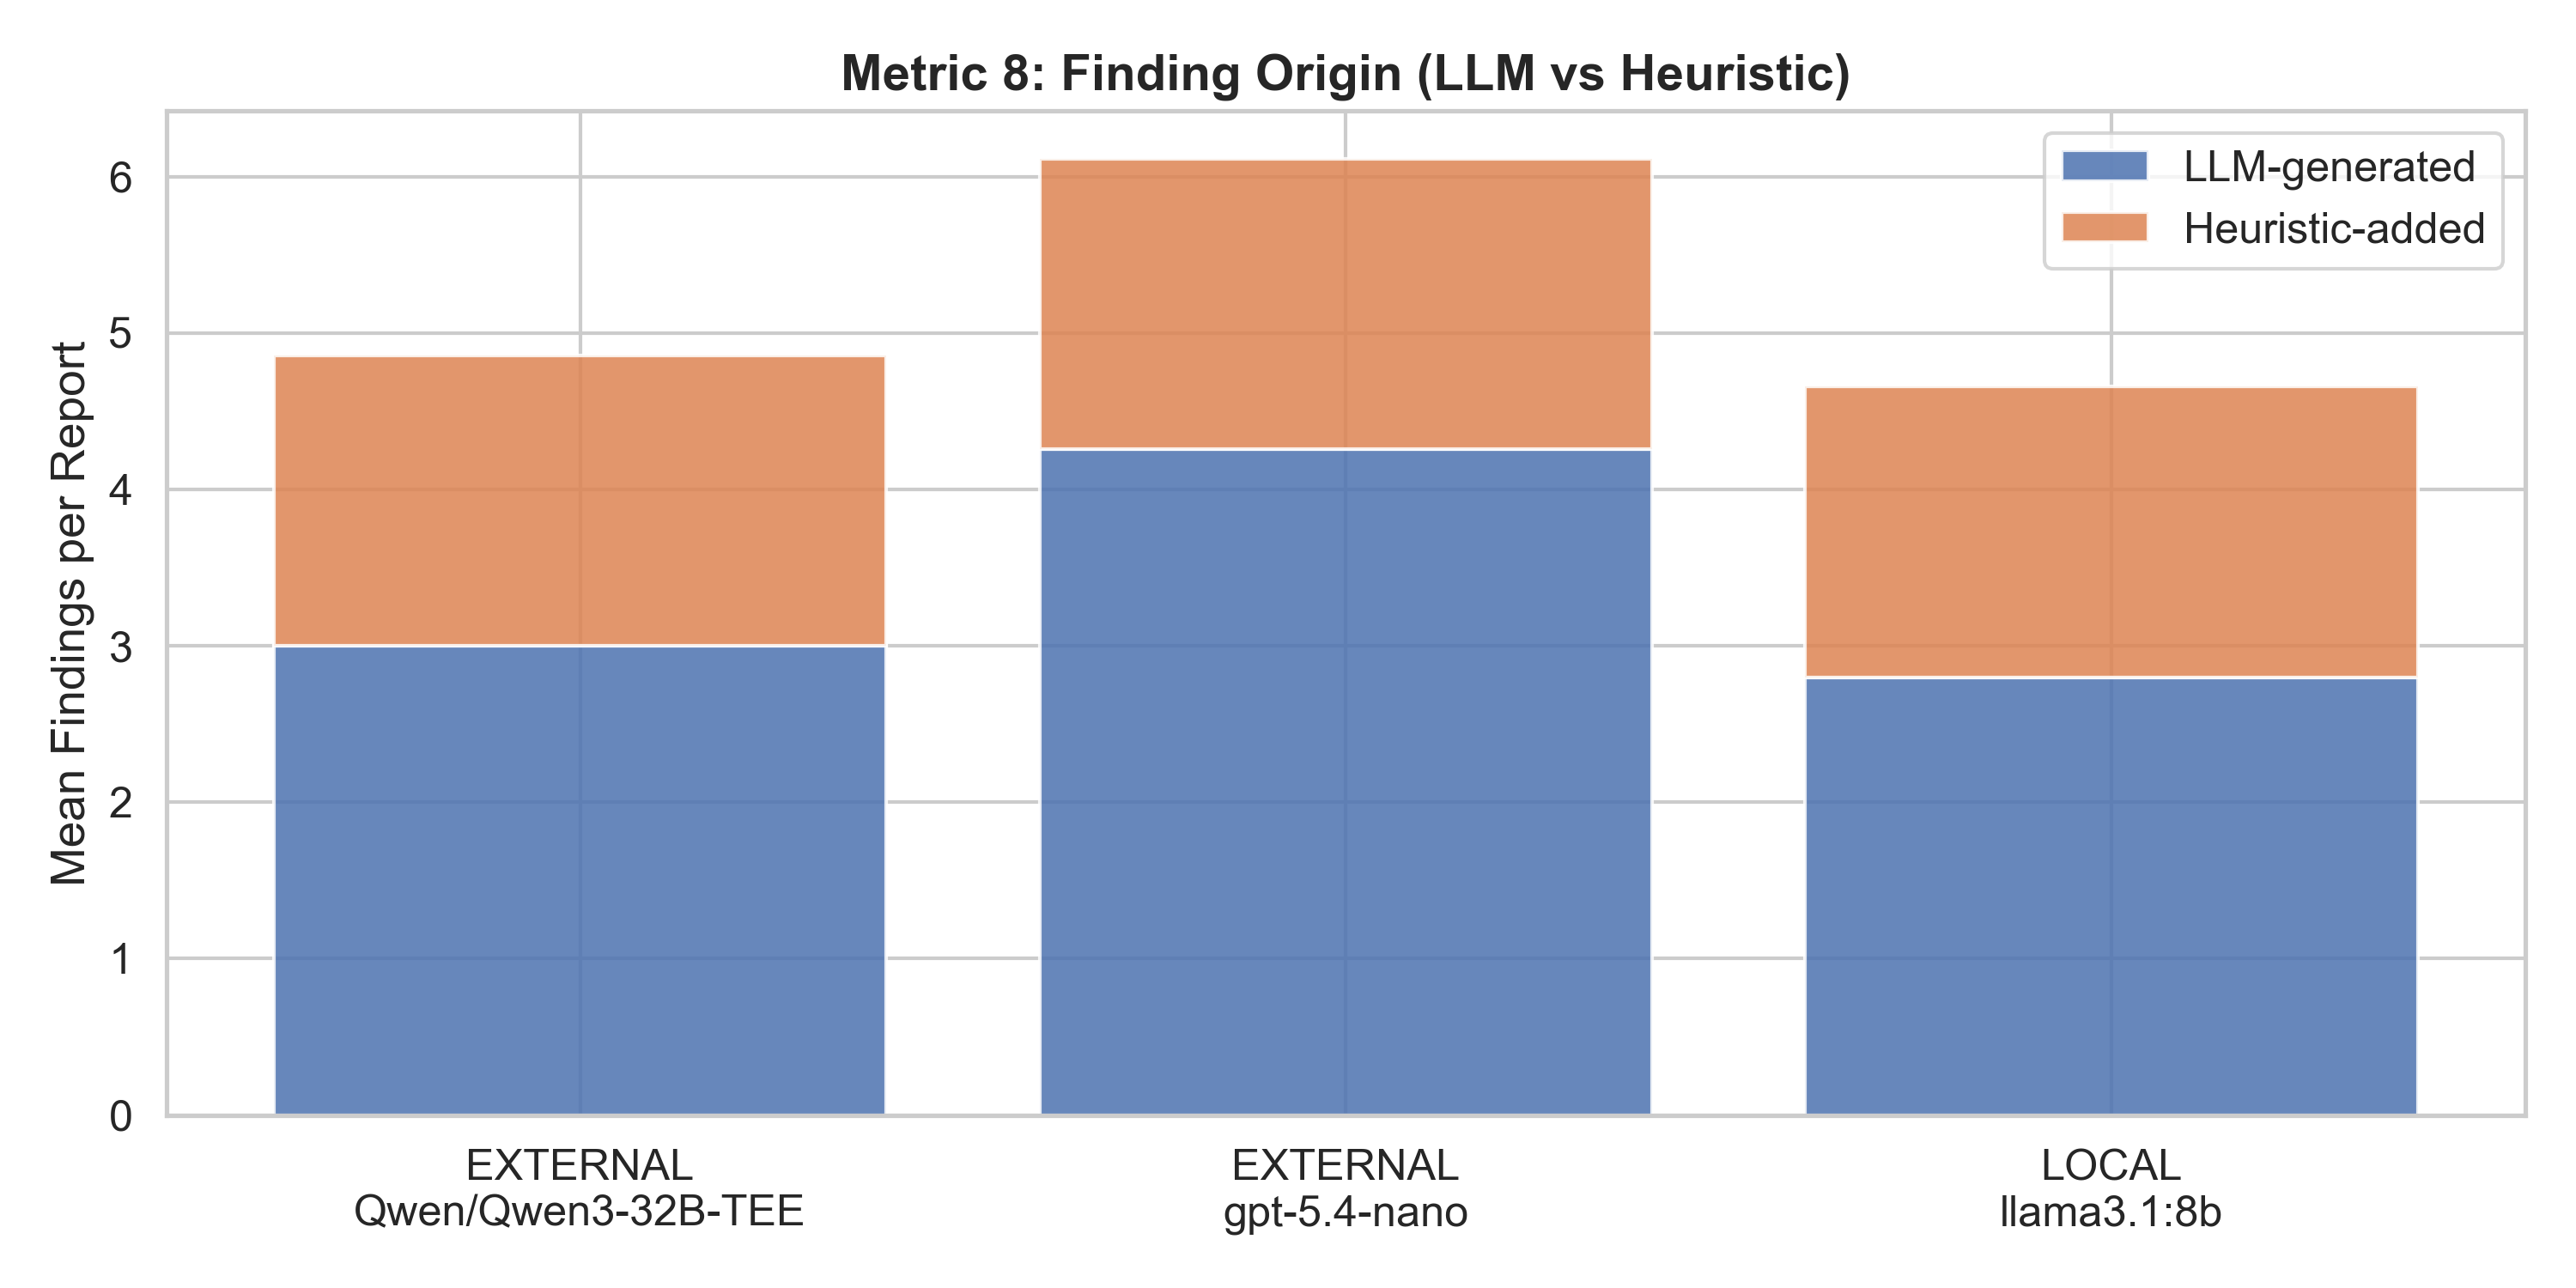
\includegraphics[width=1.0\textwidth]{src/findings_origin.png}
    \caption{Stacked contribution of LLM-originated and heuristic-injected findings per report.}
    \label{fig:findings_origin}
\end{figure}
 
\begin{table}[!ht]
    \centering
    {\footnotesize
        \begin{tabular}{|l|l|r|r|r|r|r|r|}
        \hline
            \textbf{Provider} & \textbf{Model} & \textbf{Runs} & \textbf{Mean LLM} & \textbf{Mean Heur.} & \textbf{Mean Total} & \textbf{LLM (\%)} & \textbf{Heur.\ (\%)} \\ \hline
            EXTERNAL & Qwen/Qwen3-32B-TEE & 35 & 3.00 & 1.86 & 4.86 & 61.8 & 38.2 \\ \hline
            EXTERNAL & gpt-5.4-nano       & 35 & 4.26 & 1.86 & 6.11 & 69.6 & 30.4 \\ \hline
            LOCAL    & llama3.1:8b        & 35 & 2.80 & 1.86 & 4.66 & 60.1 & 39.9 \\ \hline
        \end{tabular}
    }
    \caption{Finding origin: mean counts of LLM-generated versus heuristic-added findings per report.}
    \label{tab:findings_origin}
\end{table}
 
The findings-origin split is the single most informative analytical metric in this evaluation, because it quantifies how much genuine analytical work the LLM is contributing relative to the deterministic rule engine. GPT-5.4-nano produces an average of 4.26 LLM-originated findings per report, Qwen3-32B produces 3.00, and the local LLaMA 3.1:8b produces 2.80. The absolute number of heuristic findings is essentially constant across providers (1.86 in every case), which is expected --- heuristics fire on the same metric thresholds regardless of which LLM was called, but the \textit{share} of the final report attributable to the LLM ranges from 60\% (LLaMA) to 70\% (GPT). The local model's findings are not qualitatively worse, but it produces roughly 40\% of a report by rules alone, which weakens the case for the LLM doing the analytical lifting. Qwen3-32B lands in an interesting middle position: it generates only modestly more LLM findings than the local model on average, but its outputs are structured and formatted far more reliably (Section~\ref{sec:results_structural}), suggesting that its advantage over LLaMA is more about consistency and conformance than raw analytical breadth.
 
\subsection{Response Length Distribution}
 
\begin{figure}[h]
    \centering
    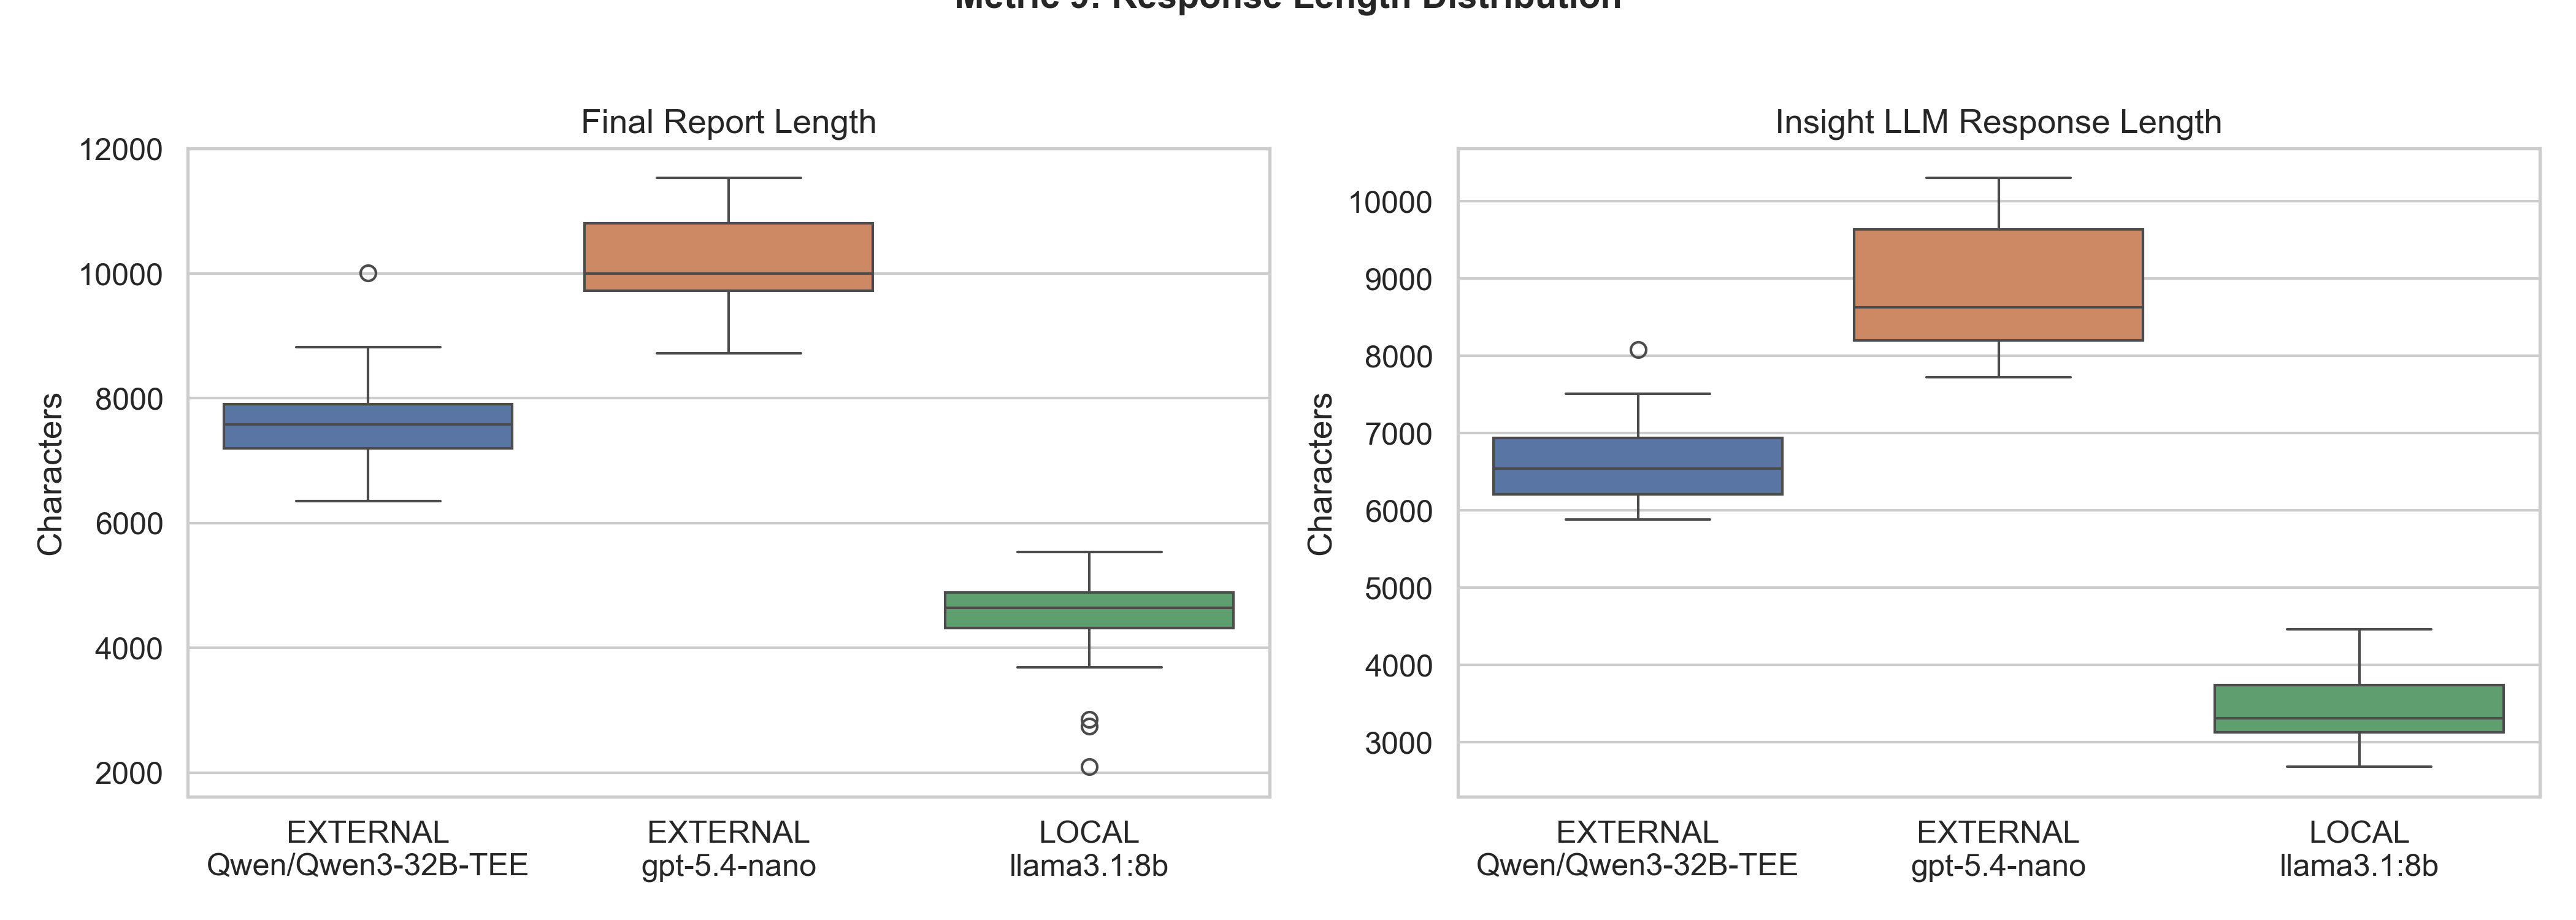
\includegraphics[width=1.0\textwidth]{src/response_length_distribution.png}
    \caption{Final report length and raw insight LLM response length distributions.}
    \label{fig:response_length_distribution}
\end{figure}
 
Report length reinforces the findings-origin pattern. GPT-5.4-nano produces the longest reports at a mean of 10{,}190 characters, Qwen3-32B averages 7{,}613, and LLaMA 3.1:8b produces substantially shorter reports at a mean of 4{,}513 characters --- less than half the length of GPT's output. The raw insight response (before Markdown rendering) follows the same ordering. Length alone is not a quality signal, but combined with the lower LLM-finding count, it suggests that the local model is producing more compressed analysis rather than simply being more concise about the same content.
 
\section{Operational Performance Metrics}
\label{sec:results_operational}
 
\subsection{Latency}
\label{sec:latency_results}
 
\begin{figure}[h]
    \centering
    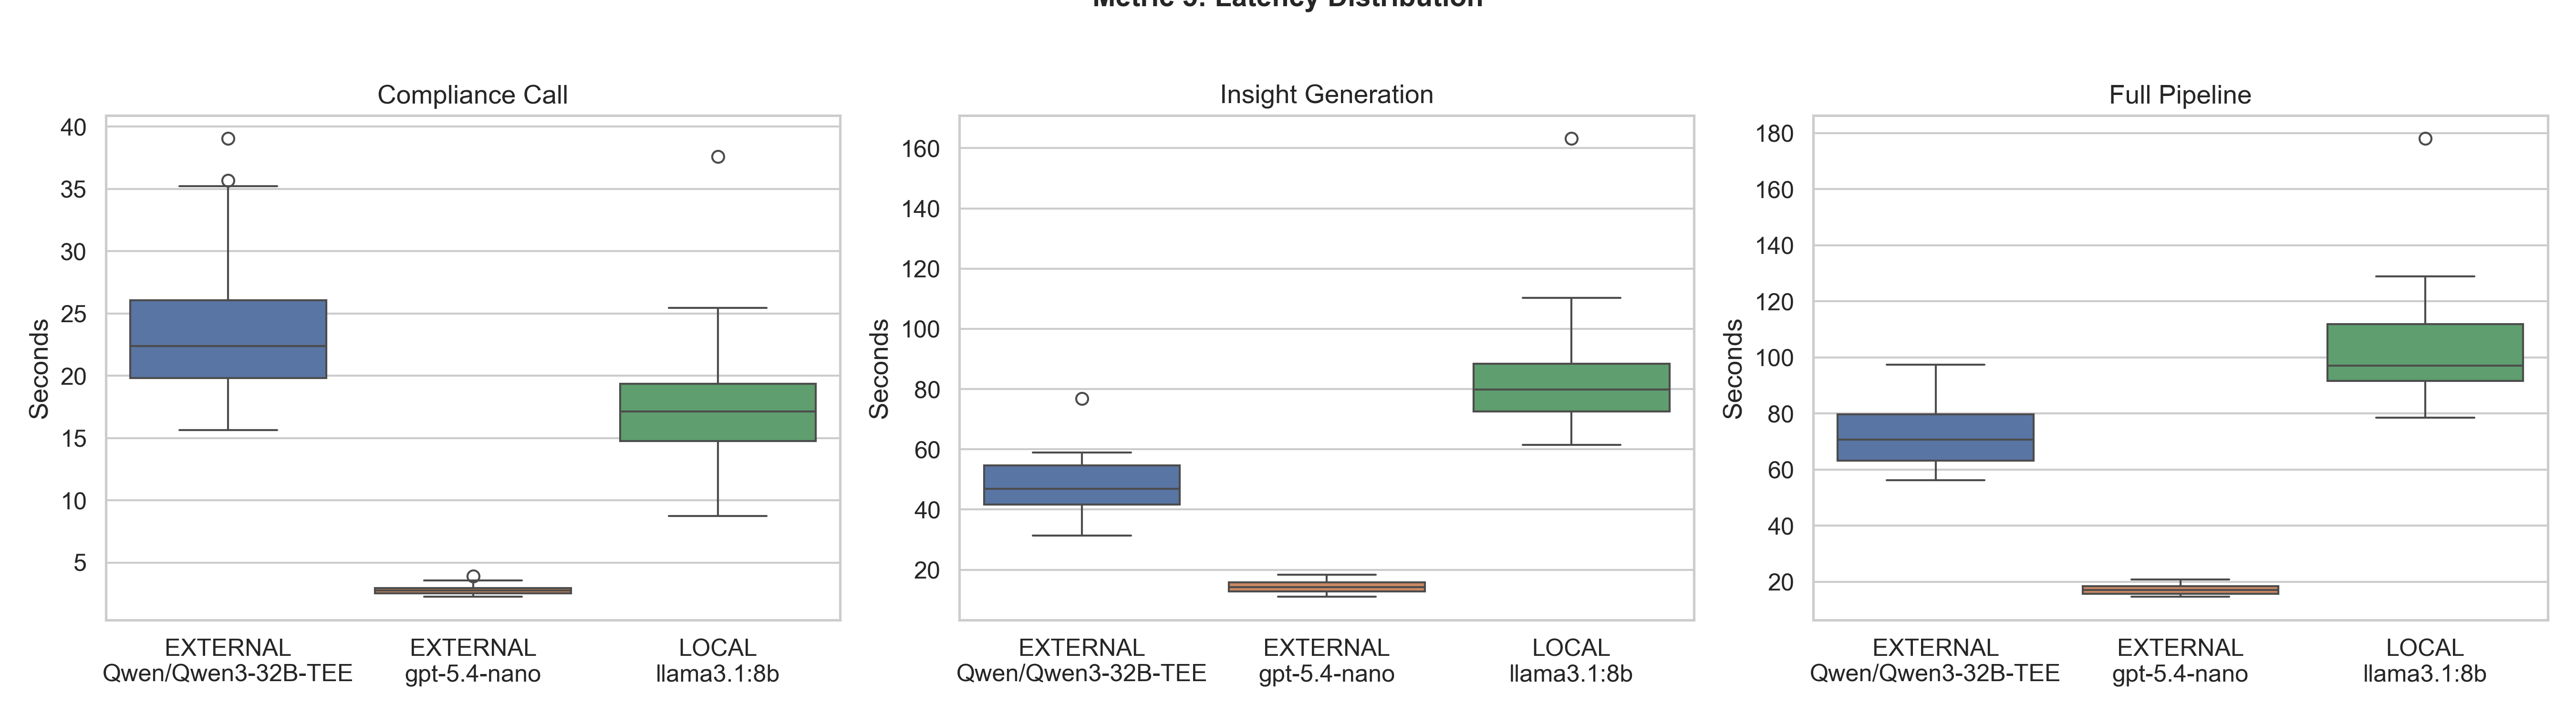
\includegraphics[width=1.0\textwidth]{src/latency_comparison.png}
    \caption{Latency distribution for the compliance call, insight call, and full pipeline, by provider and model.}
    \label{fig:latency_distribution}
\end{figure}
 
\begin{table}[!ht]
    \centering
    {\footnotesize
        \begin{tabular}{|l|l|l|r|r|r|r|r|r|}
        \hline
            \textbf{Metric} & \textbf{Provider} & \textbf{Model} & \textbf{n} & \textbf{Mean} & \textbf{Std} & \textbf{Median} & \textbf{Min} & \textbf{Max} \\ \hline
            Compliance Call (s) & EXTERNAL & Qwen/Qwen3-32B-TEE & 35 &  23.43 &  5.75 &  22.37 & 15.64 &  39.07 \\ \hline
            Compliance Call (s) & EXTERNAL & gpt-5.4-nano       & 35 &   2.77 &  0.36 &   2.76 &  2.25 &   3.91 \\ \hline
            Compliance Call (s) & LOCAL    & llama3.1:8b        & 35 &  17.67 &  5.37 &  17.15 &  8.73 &  37.62 \\ \hline
            Insight LLM (s)     & EXTERNAL & Qwen/Qwen3-32B-TEE & 35 &  48.09 &  8.66 &  46.93 & 31.39 &  76.83 \\ \hline
            Insight LLM (s)     & EXTERNAL & gpt-5.4-nano       & 35 &  14.40 &  1.95 &  14.21 & 10.98 &  18.35 \\ \hline
            Insight LLM (s)     & LOCAL    & llama3.1:8b        & 35 &  83.89 & 18.66 &  79.93 & 61.49 & 163.30 \\ \hline
            Full Pipeline (s)   & EXTERNAL & Qwen/Qwen3-32B-TEE & 35 &  71.56 & 10.41 &  70.67 & 56.29 &  97.35 \\ \hline
            Full Pipeline (s)   & EXTERNAL & gpt-5.4-nano       & 35 &  17.22 &  1.84 &  17.07 & 14.60 &  20.77 \\ \hline
            Full Pipeline (s)   & LOCAL    & llama3.1:8b        & 35 & 101.61 & 18.96 &  97.06 & 78.57 & 178.16 \\ \hline
        \end{tabular}
    }
    \caption{Latency statistics at the compliance call, insight call, and full pipeline levels.}
    \label{tab:latency_stats}
\end{table}
 
GPT-5.4-nano is the clear operational winner, completing the full pipeline in a mean of 17.2~seconds with a standard deviation of just 1.8~seconds, remarkably stable. Qwen3-32B averages 71.6~seconds, and the local LLaMA runs take 101.6~seconds on average, roughly 5.9$\times$ slower than GPT. The dominant cost for every provider is the insight call: it accounts for over 60\% of wall-clock time in every configuration. For an operator running many evaluation windows, the GPT latency profile is close to interactive; the local model's latency profile is closer to a background job. The local model also shows the largest absolute variation (standard deviation of 19.0~seconds, and a worst-case run of 178~seconds), which reflects cold-start and resource-contention effects on the Ollama container rather than a property of the model itself.
 
\subsection{Token and Cost Estimation}
 
\begin{table}[!ht]
    \centering
    {\footnotesize
        \begin{tabular}{|l|l|r|r|r|r|}
        \hline
            \textbf{Provider} & \textbf{Model} & \textbf{Runs} & \textbf{Mean input tok.} & \textbf{Mean output tok.} & \textbf{Mean total tok.} \\ \hline
            EXTERNAL & Qwen/Qwen3-32B-TEE & 35 & 2{,}741.4 & 2{,}332.1 & 5{,}073.5 \\ \hline
            EXTERNAL & gpt-5.4-nano       & 35 & 2{,}744.9 & 2{,}472.9 & 5{,}217.7 \\ \hline
            LOCAL    & llama3.1:8b        & 35 & 2{,}744.9 & 1{,}048.6 & 3{,}793.4 \\ \hline
        \end{tabular}
    }
    \caption{Estimated token usage per run (character-based $\div 4$ heuristic).}
    \label{tab:token_estimation}
\end{table}
 
Input-token counts are essentially identical across all three models (around 2{,}740 tokens), which is expected because the same prompts are constructed from the same metrics dictionary. The output side is where the models diverge sharply: the two external models produce about 2{,}300--2{,}500 output tokens per run, while the local model produces just over 1{,}000 --- less than half. This output-token gap is entirely consistent with the report-length and LLM-findings-count results, and it quantifies the ``compressed analysis'' pattern observed earlier. Monetary cost is not meaningful to compare here since the local deployment has no per-call API cost and both external endpoints were accessed via a shared development tier with pricing that does not generalise to production rates; the table therefore reports token volume only.
 
\subsection{Cross-Run Consistency}
 
\begin{table}[!ht]
    \centering
    {\footnotesize
        \begin{tabular}{|l|l|r|r|r|}
        \hline
            \textbf{Provider} & \textbf{Model} & \textbf{Total findings CV} & \textbf{LLM findings CV} & \textbf{Report length CV} \\ \hline
            EXTERNAL & Qwen/Qwen3-32B-TEE & 0.000 & 0.000 & 0.084 \\ \hline
            EXTERNAL & gpt-5.4-nano       & 0.041 & 0.061 & 0.052 \\ \hline
            LOCAL    & llama3.1:8b        & 0.151 & 0.247 & 0.147 \\ \hline
        \end{tabular}
    }
    \caption{Mean coefficient of variation across repeated runs on identical input windows (lower is more consistent).}
    \label{tab:consistency}
\end{table}
 
With five repeated runs per window per model, cross-run consistency can now be measured precisely. Qwen3-32B is the most deterministic model: its coefficient of variation on both total-findings and LLM-findings counts is zero, meaning it produced exactly the same number of findings on every repeated run. GPT-5.4-nano is close behind, with small but non-zero CVs (0.041 and 0.061). The local model is a clear outlier: its LLM-findings CV of 0.247 indicates that repeated runs on identical input can produce materially different finding counts, and its report-length CV of 0.147 means that report size varies by roughly 15\% from run to run. For compliance documentation, where reproducibility across runs is a regulatory expectation in many audit contexts, this is the weakness that is hardest to design around.
 
\section{Statistical Testing}
\label{sec:results_statistical_testing}
 
\subsection{Mann--Whitney U test}
 
\begin{table}[!ht]
    \centering
    {\footnotesize
        \begin{tabular}{|l|r|r|r|r|r|l|r|l|}
        \hline
            \textbf{Metric} & \textbf{EXT mean} & \textbf{EXT std} & \textbf{LOCAL mean} & \textbf{LOCAL std} & \textbf{p} & \textbf{Sig.} & \textbf{Cohen's d} & \textbf{Effect} \\ \hline
            Insight Latency (s)   &   31.25 &   18.08 &   83.90 &   18.66 & 0.0000 & Yes & -2.88 & Large  \\ \hline
            Pipeline Latency (s)  &   44.39 &   28.36 &  101.61 &   18.96 & 0.0000 & Yes & -2.23 & Large  \\ \hline
            Schema Conformance    &    1.00 &    0.00 &    0.91 &    0.28 & 0.0138 & Yes &  0.52 & Medium \\ \hline
            Total Findings        &    5.49 &    0.81 &    4.66 &    0.84 & 0.0000 & Yes &  1.01 & Large  \\ \hline
            LLM Findings          &    3.63 &    0.71 &    2.80 &    0.72 & 0.0000 & Yes &  1.17 & Large  \\ \hline
            Report Length (chars) & 8901.87 & 1486.74 & 4513.20 &  754.23 & 0.0000 & Yes &  3.40 & Large  \\ \hline
        \end{tabular}
    }
    \caption{Mann--Whitney U comparisons between pooled EXTERNAL and LOCAL providers ($n = 70$ and $n = 35$ respectively). A positive Cohen's $d$ means the external models score higher on that metric.}
    \label{tab:mann_whitney}
\end{table}
 
With the larger sample, all six compared metrics now differ significantly between the local and pooled external providers at the $p < 0.05$ threshold. Five of the six differences are statistically significant at $p < 0.0001$ with large effect sizes (Cohen's $|d| > 1.0$): the local model is substantially slower on both the insight call and the full pipeline, produces fewer total and LLM-originated findings, and writes much shorter reports. The schema-conformance comparison, which narrowly missed significance at the earlier sample size, now reaches $p = 0.014$ with a medium effect size ($d = 0.52$); this resolves a previously ambiguous result and confirms that the 91.4\% local conformance rate is genuinely lower than the external models' 100\%, not merely a noisy reflection of the small sample. Across the board, the statistical testing moves the local--versus--external gap from a suggestive pattern to a firmly established empirical finding.
 
\section{LLM-as-a-Judge Quality Evaluation}
\label{sec:results_judge}

This section presents the LLM-as-a-Judge evaluation defined in Section~\ref{sec:llm_judge_methodology}. The evaluation was applied to a stratified sub-sample of 36 reports (12 per source model, balanced across the seven 90-day reporting windows; see Section~\ref{sec:judge_sampling}). Two judges: Claude (Anthropic) and GPT (OpenAI), scored each report on four 1--5 Likert dimensions, yielding 288 rubric scores in total, plus a separate 36-row access-control coverage table produced by Claude alone.

\subsection{Rubric-Based Quality Scores}
\label{sec:judge_rubric_results}

Figure~\ref{fig:judge_scores_by_model} reports the mean Likert score for each (source model, dimension) cell, averaged across both judges. Figure~\ref{fig:judge_heatmap} presents the same data as a colour-coded heatmap to make cross-model comparisons easier.

\begin{figure}[h]
    \centering
    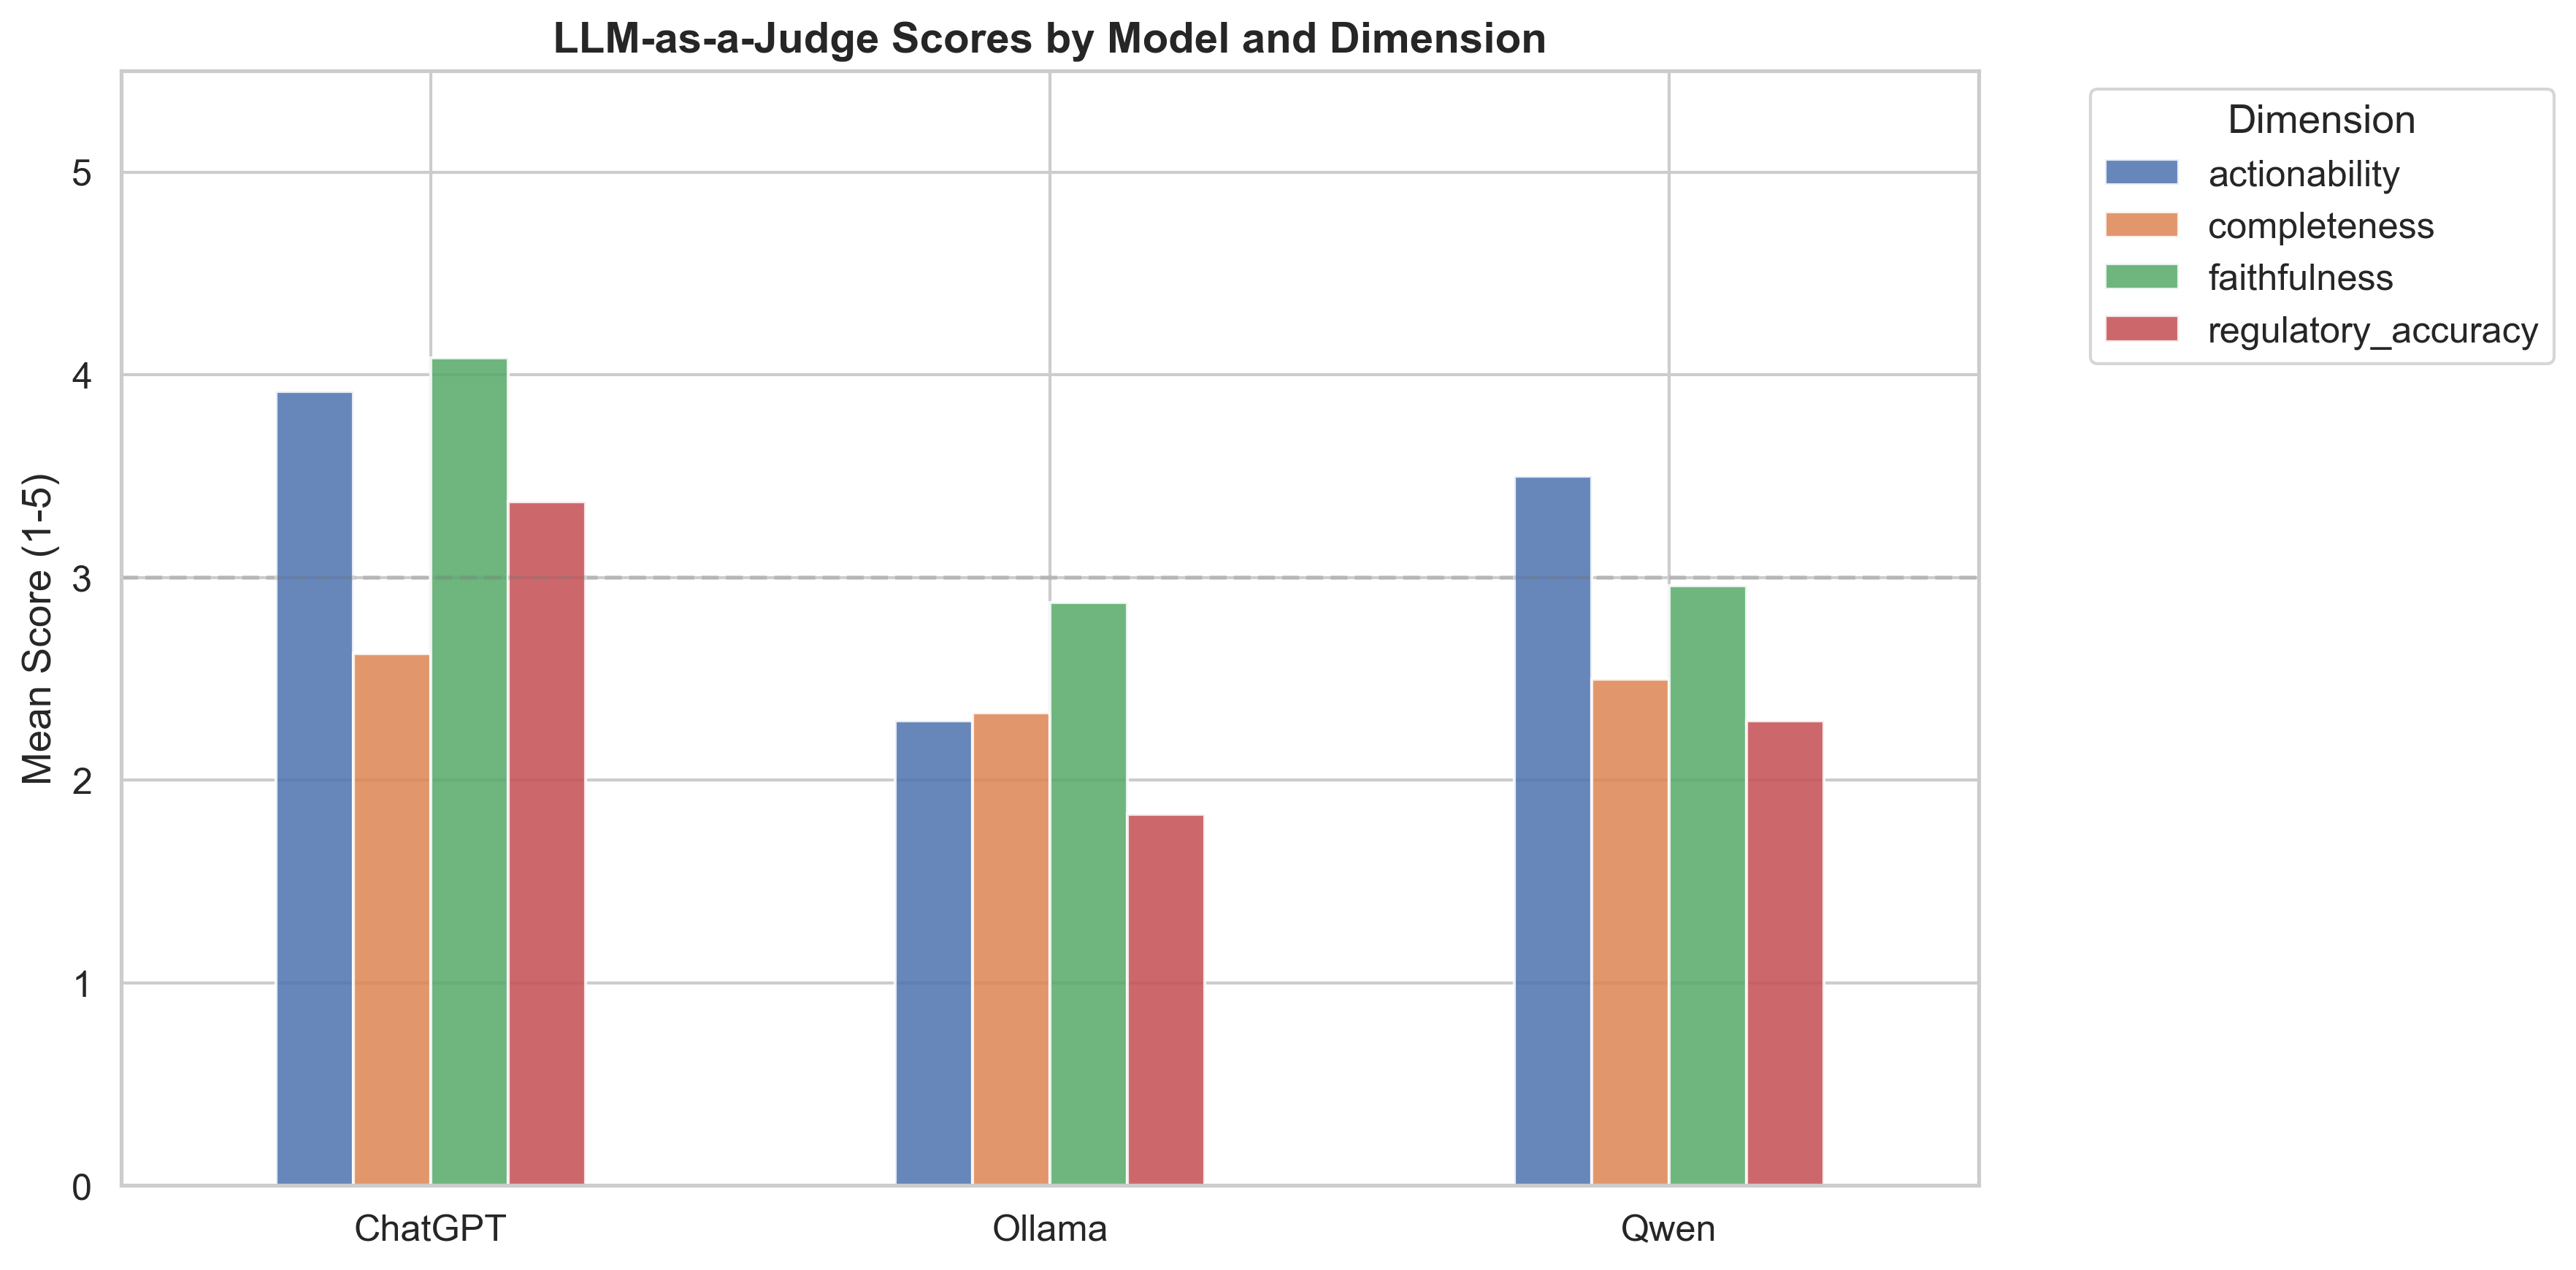
\includegraphics[width=0.95\textwidth]{src/judge_scores_by_model.png}
    \caption{Mean rubric scores across the four evaluation dimensions, averaged over both judges. The dashed grey line at 3.0 marks the rubric's ``acceptable'' threshold. In this and subsequent judge-evaluation figures, the legend label \textit{ChatGPT} refers to the \texttt{gpt-5.4-nano} configuration, and \textit{Ollama} refers to the local \texttt{llama3.1:8b} deployment.}
    \label{fig:judge_scores_by_model}
\end{figure}

\begin{figure}[h]
    \centering
    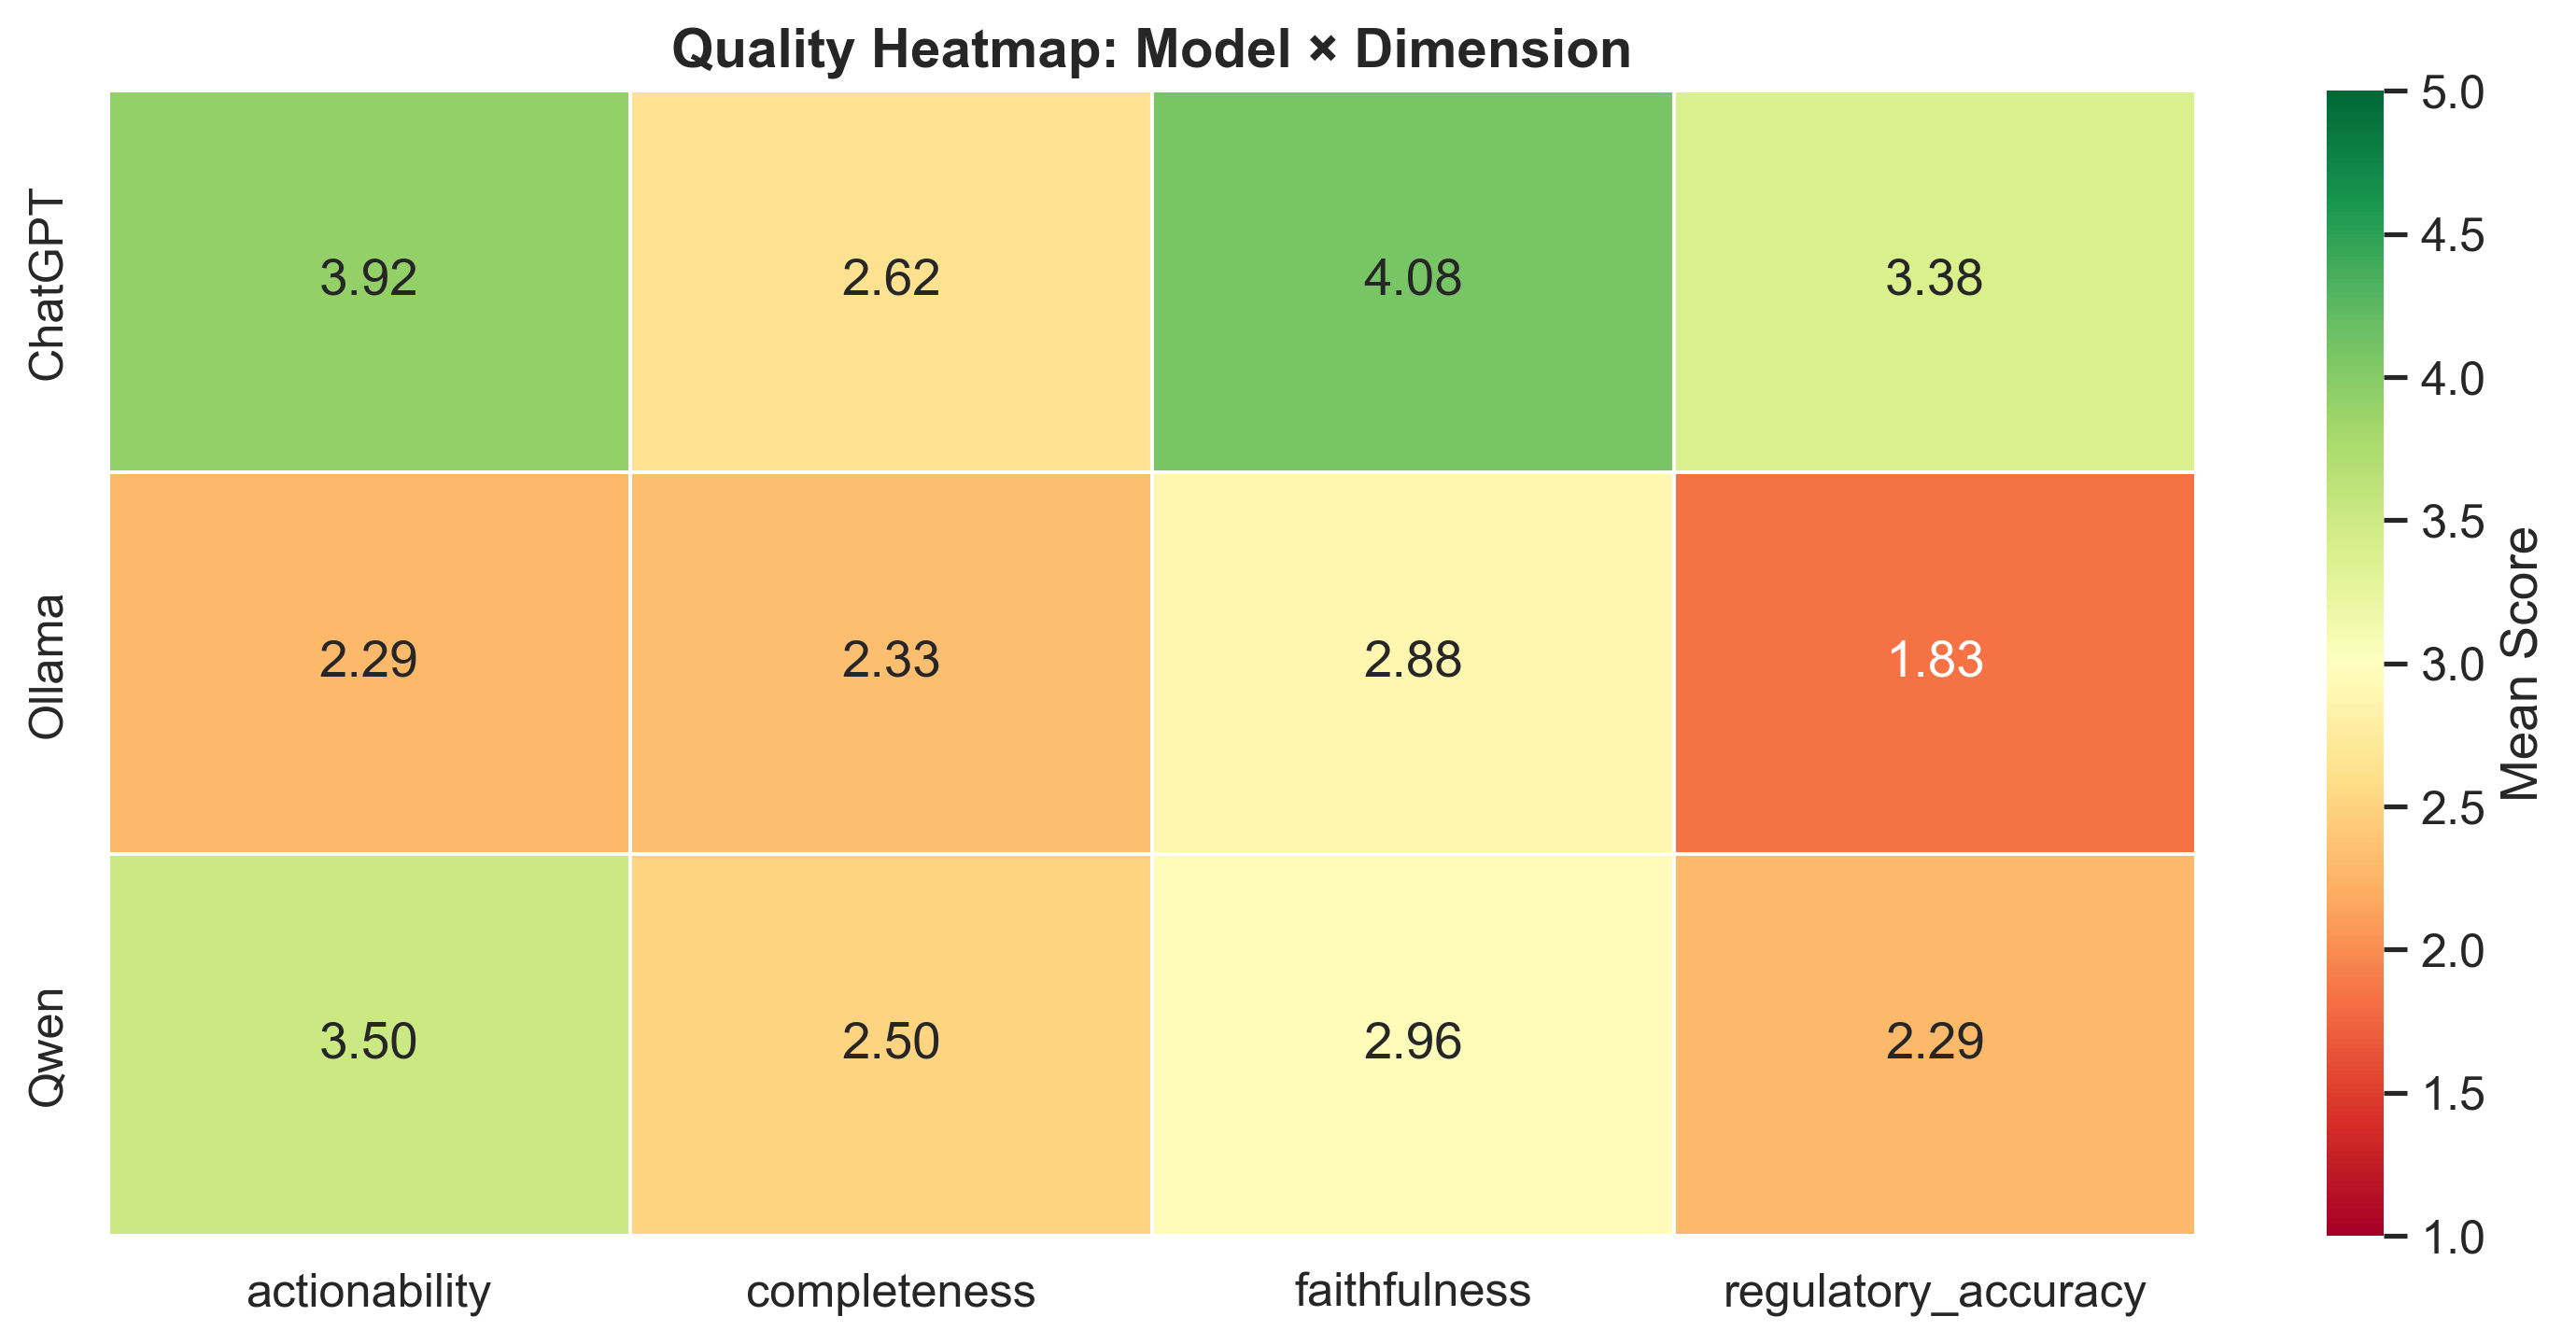
\includegraphics[width=0.85\textwidth]{src/judge_heatmap.png}
    \caption{Quality heatmap showing mean Likert scores per (source model, dimension) pair. Greener cells indicate higher quality.}
    \label{fig:judge_heatmap}
\end{figure}

The ordering across models is consistent with the automated metrics: GPT-5.4-nano is strongest on every dimension, the local LLaMA is weakest on every dimension, and Qwen3-32B sits between them. The size of the gap, however, varies sharply by dimension. \textbf{Faithfulness} shows the largest absolute spread: GPT-5.4-nano achieves a mean of 4.08, while Qwen3-32B reaches 2.96 and LLaMA 2.88. \textbf{Regulatory accuracy} shows a similar separation, with LLaMA at 1.83 (sub-acceptable) versus GPT-5.4-nano at 3.38. \textbf{Actionability} is comparatively strong for the two cloud models (3.92 GPT, 3.50 Qwen) and weak for LLaMA (2.29), suggesting that the local model produces recommendations that judges read as generic. \textbf{Completeness} is the dimension on which all three models score similarly poorly --- 2.62, 2.50, and 2.33 for GPT-5.4-nano, Qwen3-32B, and LLaMA respectively --- indicating that none of the reports comprehensively addresses the full set of relevant NIS2 Article~21(2) measures. This is consistent with the topic-coverage results presented in Section~\ref{sec:judge_topic_coverage}: every model leaves several sub-topics untouched.

\subsection{Inter-Judge Agreement and Self-Enhancement Bias}
\label{sec:judge_agreement}

Figure~\ref{fig:inter_judge_comparison} contrasts each judge's mean scores per dimension, aggregated across all source models.

\begin{figure}[h]
    \centering
    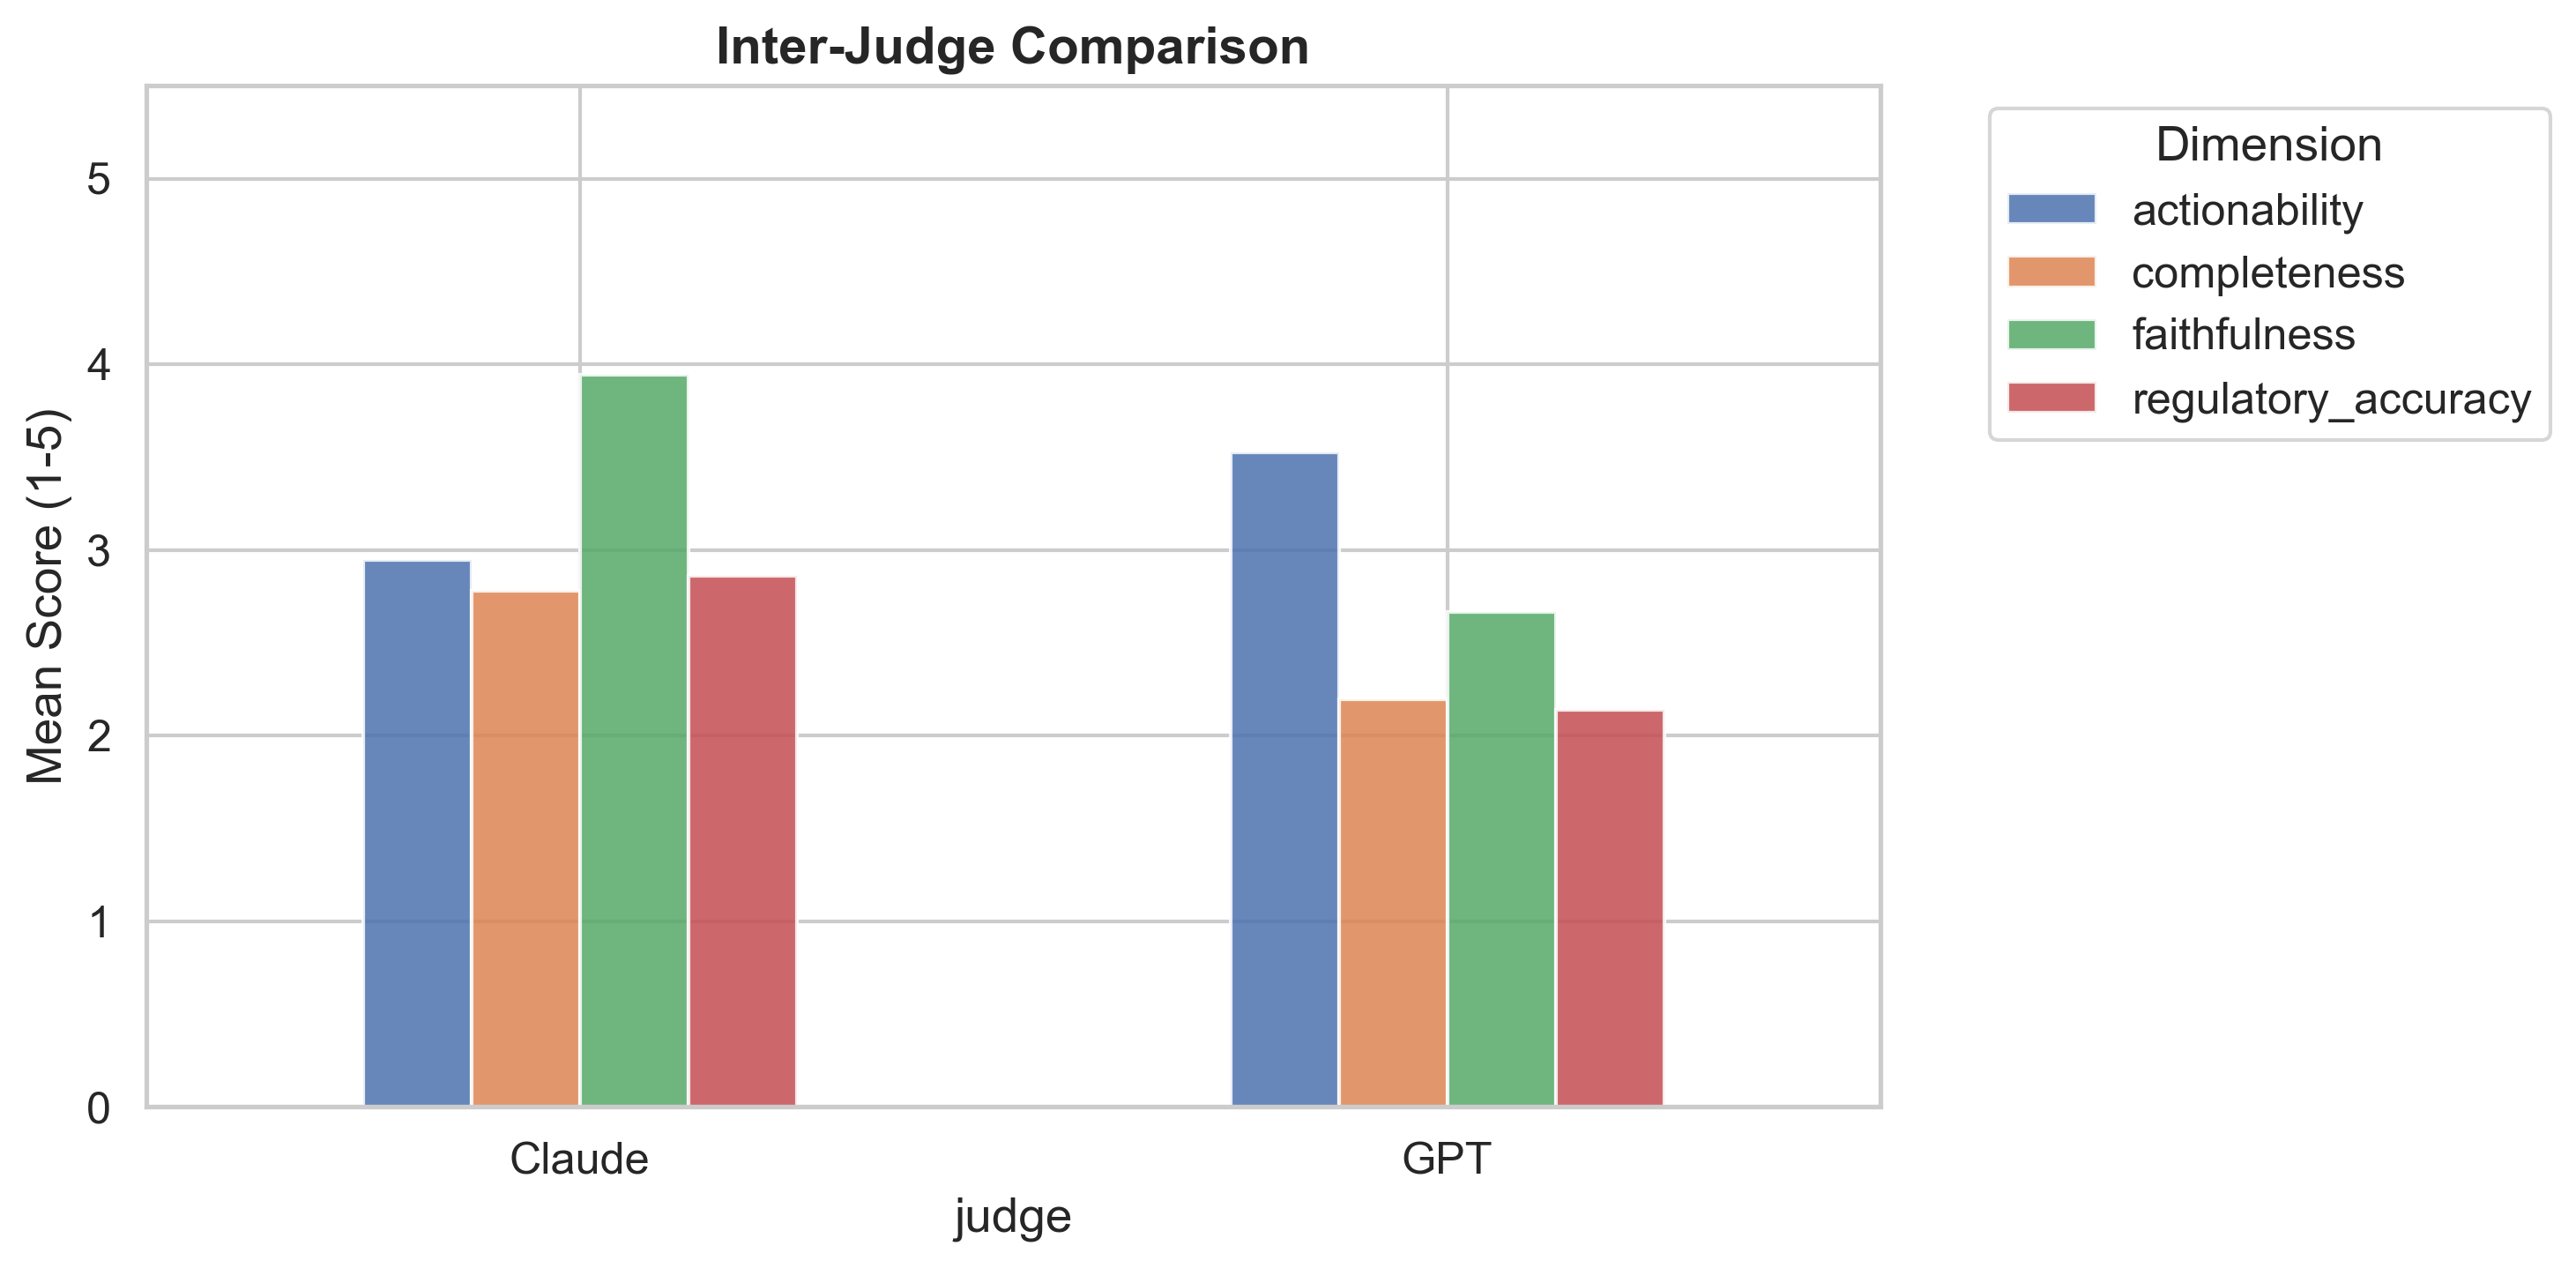
\includegraphics[width=0.85\textwidth]{src/inter_judge_comparison.png}
    \caption{Per-judge mean scores by dimension, aggregated across all three source models. Claude tends to score higher than GPT overall; the gap varies by dimension as shown.}
    \label{fig:inter_judge_comparison}
\end{figure}

The two judges show systematically different scoring tendencies. Aggregating across all source models and dimensions, Claude's mean cell score is 3.13 while GPT's is 2.63 --- a Claude-favourable mean delta of $+0.50$ on the 1--5 scale. Cohen's $\kappa$ with linear weights over the 144 matched (report, folder, dimension) pairs is $0.228$, with a Pearson correlation of $r = 0.478$. On the customary $\kappa$ scale these values indicate \textit{fair} absolute agreement between the judges, falling short of the moderate-agreement threshold of $0.40$, although both judges recover the same dimension-wise model ordering, GPT-5.4-nano $>$ Qwen3-32B $>$ LLaMA, on every dimension (Figure~\ref{fig:inter_judge_comparison}). The mismatch between consistent dimension-wise orderings and divergent absolute scores is the typical pattern reported in the LLM-as-a-judge literature\cite{ZhengMTBench2023} and is the reason the analysis below relies on \textit{relative} comparisons rather than raw averages.

The self-enhancement check yields an unexpected result. GPT scored GPT-5.4-nano's reports at a mean of 3.19, while Claude scored the same reports at 3.81 --- a delta of $-0.62$ \textit{against} GPT's own outputs. Rather than the usual self-favouring bias predicted by Zheng et al.\cite{ZhengMTBench2023}, GPT here is the more critical reviewer of its own family's writing. The plausible explanations are that GPT applies the rubric more strictly than Claude across the board (consistent with its lower overall mean) or that it is more sensitive to the specific failure modes that GPT-5.4-nano exhibits. The practical implication for this evaluation is the same in either case: pooling both judges' scores for GPT-5.4-nano reports would understate their quality relative to the other models, because LLaMA and Qwen do not have a same-vendor judge applying equivalently strict scoring. The reported headline scores in Section~\ref{sec:judge_bias_adjusted} are therefore \textit{bias-adjusted}, dropping GPT's ratings on GPT-5.4-nano reports while retaining both judges for LLaMA and Qwen3-32B.

\subsection{Bias-Adjusted Comparison and Statistical Tests}
\label{sec:judge_bias_adjusted}

Table~\ref{tab:judge_bias_adjusted} reports the bias-adjusted mean score per (source model, dimension), together with an overall mean across the four dimensions.

\begin{table}[!ht]
    \centering
    {\footnotesize
    \begin{tabular}{|l|c|c|c|c|c|}
    \hline
    \textbf{Source Model} & \textbf{Reg.\ Accuracy} & \textbf{Completeness} & \textbf{Faithfulness} & \textbf{Actionability} & \textbf{Overall} \\ \hline
    GPT-5.4-nano       & 3.83 & 2.83 & 4.75 & 3.83 & \textbf{3.81} \\ \hline
    Qwen3-32B-TEE      & 2.29 & 2.50 & 2.96 & 3.50 & 2.81          \\ \hline
    LLaMA 3.1:8b       & 1.83 & 2.33 & 2.88 & 2.29 & 2.33          \\ \hline
    \end{tabular}
    }
    \caption{Bias-adjusted Likert scores. GPT's ratings on GPT-5.4-nano outputs are dropped; the other two source models retain both judges' scores. The Overall column is the mean of the four dimensions.}
    \label{tab:judge_bias_adjusted}
\end{table}

A Mann--Whitney U test compares the bias-adjusted scores between LOCAL (LLaMA via Ollama) and pooled EXTERNAL (GPT-5.4-nano + Qwen3-32B) on each dimension. Results are reported in Table~\ref{tab:judge_mann_whitney}. All four dimensions show a statistically significant gap at $p < 0.05$. Two dimensions reach $p < 0.001$ with large effect sizes (Cohen's $|d| > 0.8$): actionability ($d = -2.73$), the largest effect, and regulatory accuracy ($d = -1.29$). The remaining two dimensions show medium effects: faithfulness ($d = -0.66$) and completeness ($d = -0.57$). The pattern is consistent with the automated-metric findings in Table~\ref{tab:mann_whitney}: every quality dimension that can be measured shows the local model trailing the cloud models, often by a substantial margin.

\begin{table}[!ht]
    \centering
    {\footnotesize
    \begin{tabular}{|l|c|c|c|c|c|l|}
    \hline
    \textbf{Dimension} & \textbf{LOCAL mean} & \textbf{EXT mean} & \textbf{$p$} & \textbf{Sig.} & \textbf{Cohen's $d$} & \textbf{Effect} \\ \hline
    Regulatory Accuracy & 1.83 & 2.81 & 0.0000 & Yes & $-1.29$ & Large  \\ \hline
    Completeness        & 2.33 & 2.61 & 0.0374 & Yes & $-0.57$ & Medium \\ \hline
    Faithfulness        & 2.88 & 3.56 & 0.0225 & Yes & $-0.66$ & Medium \\ \hline
    Actionability       & 2.29 & 3.61 & 0.0000 & Yes & $-2.73$ & Large  \\ \hline
    \end{tabular}
    }
    \caption{Mann--Whitney U comparison of bias-adjusted Likert scores between LOCAL and pooled EXTERNAL providers. A negative Cohen's $d$ means LOCAL scored lower than the external pool.}
    \label{tab:judge_mann_whitney}
\end{table}

\subsection{Access Control Topic Coverage}
\label{sec:judge_topic_coverage}

The coverage metric counts how many of twelve access-control sub-topics each report substantively addresses. Recall from Section~\ref{sec:access_control_coverage} that, unlike the rubric-based dimensions, coverage is scored by a single judge (Claude) rather than the full panel. Aggregate results are shown in Figure~\ref{fig:access_control_coverage}, and the per-topic breakdown in Figure~\ref{fig:topic_coverage_heatmap}.

\begin{figure}[h]
    \centering
    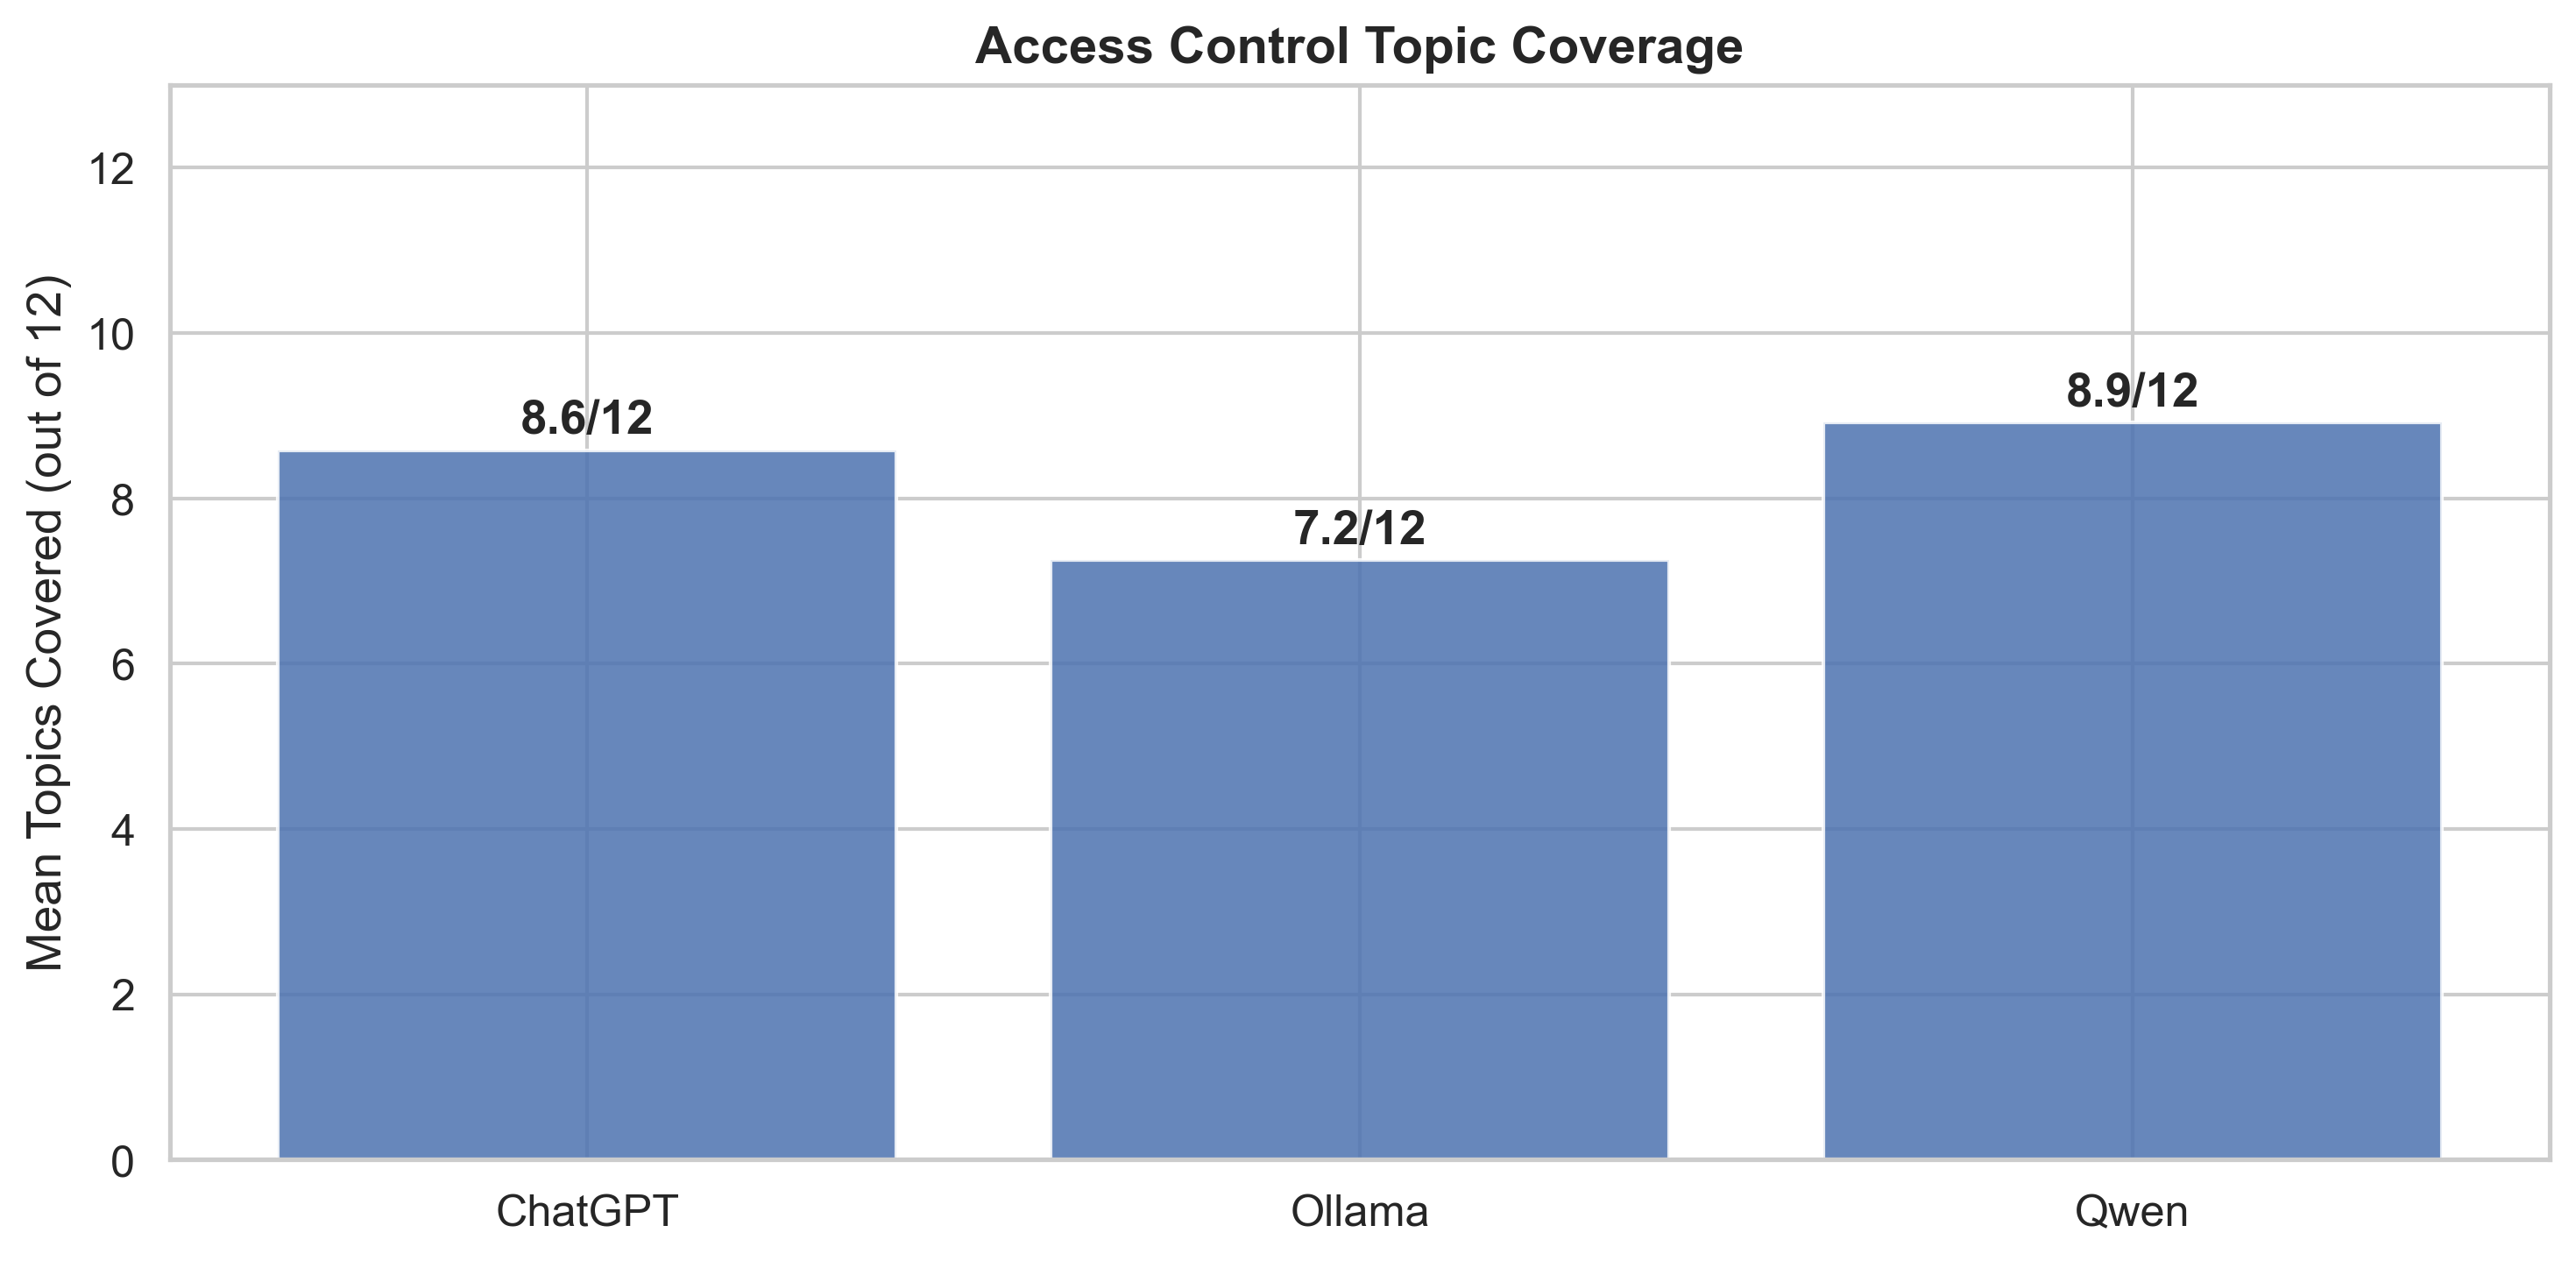
\includegraphics[width=0.85\textwidth]{src/access_control_coverage.png}
    \caption{Mean number of access-control sub-topics covered per report (out of 12).}
    \label{fig:access_control_coverage}
\end{figure}

\begin{figure}[h]
    \centering
    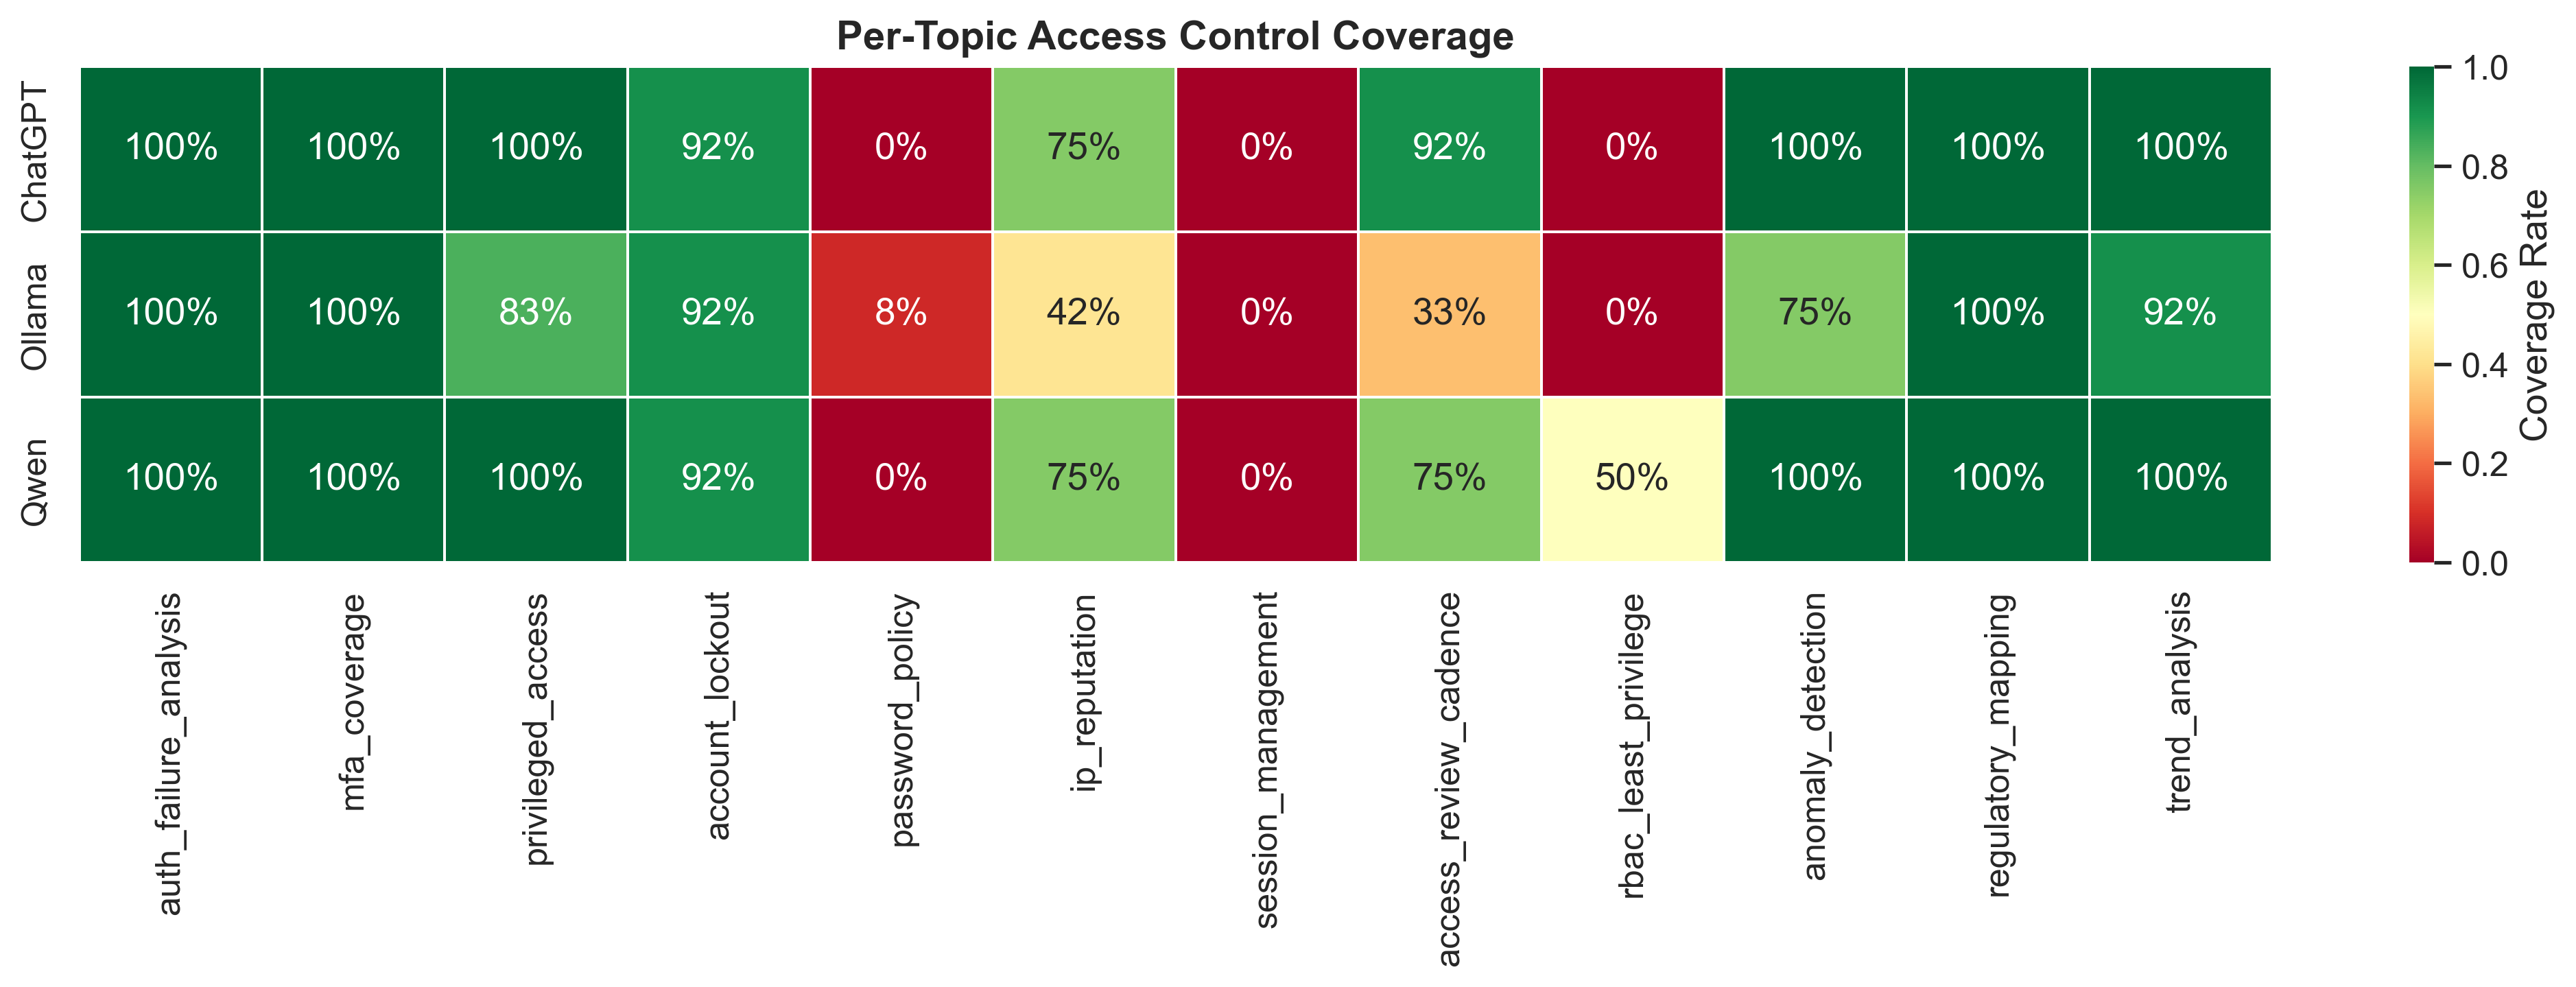
\includegraphics[width=1.0\textwidth]{src/topic_coverage_heatmap.png}
    \caption{Per-topic coverage rates across the three source models. Cells show the proportion of reports that substantively address each sub-topic.}
    \label{fig:topic_coverage_heatmap}
\end{figure}

Aggregate coverage is broadly comparable for the two cloud models, Qwen3-32B reaches 8.92/12 on average and GPT-5.4-nano 8.58/12, with the local LLaMA noticeably behind at 7.25/12. The inversion of the rubric ordering (Qwen edges GPT on coverage breadth even though GPT scored higher on every Likert dimension) is itself informative: Qwen's reports touch on a slightly wider set of sub-topics, but the depth or grounding of those mentions, as scored on faithfulness and regulatory accuracy, is weaker than GPT's. The local LLaMA also shows the largest within-model variance (standard deviation 1.14 vs.\ 0.67 for GPT-5.4-nano), which mirrors its higher cross-run variance on the automated metrics.

The per-topic heatmap (Figure~\ref{fig:topic_coverage_heatmap}) reveals where the gaps are. Four topics are addressed in essentially every report by every model: authentication failure analysis, MFA coverage, regulatory mapping (i.e.\ the reports always cite NIS2 articles), and trend analysis. A second tier --- privileged access review, account lockout policies, and anomalous login detection --- is covered by the cloud models almost universally and by LLaMA most of the time (83\% on privileged access, 75\% on anomaly detection), with access-review cadence the main weakness for LLaMA (33\%) compared with both cloud models. Three topics are systematically under-covered by every model: \textit{password policy compliance} (covered by 0--8\% of reports), \textit{role-based access control / least-privilege analysis} (0\% for LLaMA and GPT-5.4-nano; 50\% for Qwen), and \textit{session management} (0\% across all models). These three blind spots correspond to controls that are not directly evidenced in the underlying RBA dataset --- the dataset captures authentication events but not RBAC role assignments, password rotation, or session timeouts, so the gap is best read as a limitation of the input data rather than a model failure. It does, however, mark a clear scope boundary for the system as currently configured: a complete NIS2 Article~21(2)(i)--(j) report would require additional log feeds to evidence those three controls.

\section{Summary Comparison}
\label{sec:results_summary}
 
\begin{table}[!ht]
    \centering
    {\footnotesize
        \begin{tabular}{|l|c|c|c|}
        \hline
            \textbf{Provider}                       & EXTERNAL            & EXTERNAL     & LOCAL        \\ \hline
            \textbf{Model}                          & Qwen/Qwen3-32B-TEE  & gpt-5.4-nano & llama3.1:8b  \\ \hline
            \textbf{Runs}                           & 35                  & 35           & 35           \\ \hline
            \textbf{JSON Parse Rate (\%)}           & 100.0               & 100.0        & 91.4         \\ \hline
            \textbf{Schema Conformance (\%)}        & 100.0               & 100.0        & 91.4         \\ \hline
            \textbf{Severity Valid (\%)}            & 100.0               & 100.0        & 100.0        \\ \hline
            \textbf{Mean Pipeline Latency (s)}      & 71.6                & 17.2         & 101.6        \\ \hline
            \textbf{Mean LLM Findings}              & 3.0                 & 4.3          & 2.8          \\ \hline
            \textbf{Mean Heuristic Findings}        & 1.9                 & 1.9          & 1.9          \\ \hline
            \textbf{Mean Tokens / Run}              & 5073                & 5218         & 3793         \\ \hline
            \textbf{Mean Report Length}             & 7613                & 10190        & 4513         \\ \hline
            \textbf{Judge Quality (overall, 1--5)}  & 2.81                & 3.81         & 2.33         \\ \hline
            \textbf{Topic Coverage (out of 12)}     & 8.92                & 8.58         & 7.25         \\ \hline
        \end{tabular}
    }
    \caption{Final comparison across all automated metrics and the LLM-as-a-Judge evaluation. The judge-quality row reports the bias-adjusted overall score from Table~\ref{tab:judge_bias_adjusted}; the topic-coverage row uses the 12 access-control sub-topics defined in Section~\ref{sec:llm_judge_methodology}.}
    \label{tab:final_comparison}
\end{table}
 
Table~\ref{tab:final_comparison} consolidates the nine automated metrics together with the LLM-as-a-Judge headline scores into a single comparison. GPT-5.4-nano is the strongest model on every quality dimension: structural, analytical, judge-rated, and dominates on latency. Qwen3-32B-TEE sits in the middle: quality comparable to GPT on structural metrics, weaker on analytical depth (3.0 vs 4.3 LLM findings), and noticeably slower (71.6~s vs 17.2~s); on the judge metrics it edges GPT slightly on topic coverage breadth (8.92 vs 8.58 of 12) but trails on the rubric quality score (2.81 vs 3.81). The local LLaMA 3.1:8b lags on every metric except tokens-per-run, where its lower output-token count reflects shorter reports rather than any efficiency win, and posts the lowest judge-quality score (2.33) and lowest topic coverage (7.25/12). The overall picture is that local deployment is structurally viable, the system works end-to-end, but the quality, consistency, and latency penalties relative to cloud-hosted models are measurable and, in several cases, large.

\chapter{Conclusion}
\label{sec:conclusion}
\section{Summary of Objectives and Contributions}
\label{sec:conclusion_summary}

This project investigated whether Generative AI can meaningfully reduce the manual burden of cybersecurity compliance documentation under the EU's NIS2 Directive\cite{NIS2Directive2023} and ISO/IEC~27001 control A.9\cite{ISO27001A9}. The four objectives set out in Chapter~\ref{chp:introduction} have all been addressed: a working data-to-text pipeline was designed and implemented; suitable open log corpora were identified and the system was evaluated against the RBA authentication dataset; structural compliance, analytical quality, and operational performance were measured across local and cloud-hosted models; and an LLM-as-a-Judge evaluation assessed whether the resulting reports are of draft-grade quality.

The principal contribution is the pipeline itself: a modular, microservice-based system that combines deterministic streaming analytics with retrieval-grounded generation, so that every numeric claim in a report is traceable to computed evidence and every regulatory claim is anchored in retrieved source text. A secondary contribution is the comparative evaluation framework, which gives organisations a reproducible basis for choosing between local privacy-preserving deployment and cloud-hosted quality, rather than relying on subjective assessment.

\section{Key Design Decisions and Their Outcomes}
\label{sec:conclusion_design_decisions}

The project's most consequential design decision was negative: the preliminary LoRA fine-tuning experiment (Section~\ref{sec:lora_experiment_eval}) showed that parameter-efficient fine-tuning on a small, hardware-constrained training set produces hallucinated regulatory content rather than disciplined compliance prose. That failure clarified the central principle of the final architecture, mainlu that fluency without grounding is dangerous in a regulatory setting, and motivated the move to a hybrid design in which deterministic analytics provide the verifiable backbone of every report, RAG retrieval anchors regulatory claims in the actual source text, and human-in-the-loop approval gates schema and metric onboarding. The result is a system in which the LLM is responsible for narration rather than for facts, which is the appropriate division of labour for compliance documentation.

\section{Evaluation Findings}
\label{sec:conclusion_findings}

The evaluation reported in Chapter~\ref{chp:eval_results} produced three findings that bear directly on the central research question. First, the system works: across 105 pipeline runs covering three model configurations and seven 90-day reporting windows, every input produced a valid, schema-conformant report, and the LLM-as-a-Judge panel consistently rated the cloud-model outputs above the rubric's ``acceptable'' threshold on the dimensions most central to compliance --- regulatory accuracy and actionability. Generative AI can therefore produce draft cybersecurity compliance documentation of genuinely useful quality, given the grounding mechanisms described above.

Second, the local-versus-cloud trade-off is real and measurable, but it is not categorical. The local LLaMA~3.1:8b deployment trailed both cloud models on every quality dimension and on every operational metric, with statistically significant gaps and large effect sizes on the dimensions that matter most. Yet the same local deployment produced structurally valid reports the great majority of the time, recovered the same ordering of issues that the cloud models did, and offered the privacy guarantees that the cloud models cannot. The choice between deployment modes is therefore a governance decision shaped by data-sovereignty requirements and tolerance for variability, not a binary judgement about whether local LLMs are ``ready''.

Third, completeness emerged as the dimension on which all three models scored similarly poorly --- a finding that points away from the LLM and toward the input. Several NIS2 Article~21 access-control sub-topics, notably session management, role-based access control, and password policy, are absent from every report not because the models could not articulate them but because the underlying RBA dataset does not evidence them. This boundary is a property of the evidence pipeline, not the generative layer, and it suggests that future improvements in compliance-report quality will come at least as much from broadening the telemetry feed as from upgrading the language model.

\section{Ethical Considerations}
\label{sec:conclusion_ethics}

Three ethical considerations follow from the work. The fluency and professional appearance of LLM-generated text creates a real risk that organisations will treat draft reports as authoritative without adequate human review; the system mitigates this through visible confidence scores and explicit AI labelling, but final responsibility for submitted documentation must remain with qualified personnel. Authentication logs and security telemetry, even when pseudonymised, can reveal patterns of user behaviour, which is why the local-deployment mode processes data on-premise via Ollama and why any use of external APIs must be governed by GDPR-aligned data-handling controls\cite{GDPR2016}. More broadly, the proliferation of AI-assisted compliance reporting risks producing documentation that is superficially well-written but substantively shallow; the deterministic grounding mechanisms in this system are intended to push against that drift, but the compliance ecosystem as a whole will need to develop verification norms appropriate to AI-assisted artefacts.

\section{Limitations}
\label{sec:conclusion_limitations}

Several limitations frame the conclusions above. The empirical evaluation is restricted to a single regulatory domain (access control under NIS2 Article~21) and a single input dataset (RBA authentication logs), so claims about generalisability to incident response, supply-chain security, or other compliance frameworks are inferred from the architecture rather than demonstrated. The local-versus-cloud comparison is similarly conditional on the three specific models tested; conclusions about ``local'' deployment depend on LLaMA~3.1:8b as the representative open-weight model and would need to be retested as that ecosystem matures. The automated metrics capture structural and operational properties rigorously but are silent on factual accuracy at the claim level, and although the LLM-as-a-Judge evaluation closes part of that gap, inter-judge agreement is only fair on the absolute scale, and the panel itself is reduced from the originally planned three judges to two. A human-expert validation study with compliance auditors remains the most direct way to confirm that judge ratings track expert intuitions about report quality. Finally, the latency variance observed for the local model reflects cold-start and resource-contention effects on a containerised consumer-grade deployment rather than an intrinsic limit of the model, so the local-versus-cloud performance gap can be expected to narrow on dedicated hardware.

\section{Future Work}
\label{sec:conclusion_future_work}

Several directions for future work emerge from this project. The most immediate extension would be to support additional compliance domains beyond access control, including incident reporting (NIS2 Article~23), supply-chain security (NIS2 Article~21(2)(d)), and vulnerability management. Each domain introduces distinct data sources and reporting requirements, providing an opportunity to test the generalisability of the pipeline architecture.

A second line of work would involve developing a semi-automated factual accuracy evaluation. By extracting numeric claims from generated reports and cross-referencing them against the input metrics dictionary, it would be possible to compute a precision metric for quantitative statements, enabling direct measurement of hallucination in the compliance context.

Third, the integration of newer and more capable local models, such as Mistral, Phi-3, or future LLaMA iterations, could help close the quality gap observed between local and external deployments. As the open-weight model ecosystem matures, the privacy-preserving deployment scenario may become increasingly competitive without sacrificing output quality.

Finally, a user study with compliance professionals and cybersecurity auditors would provide valuable qualitative feedback on the practical utility of AI-generated compliance reports. Such a study could assess whether the reports meet the expectations of regulatory reviewers, identify areas where AI-generated prose falls short of expert-written documentation, and inform further refinements to the prompt engineering and report templating strategies.
%%%%%%%%


%%%%%%%%%%%%%%%%%%%%%%
%%% Acknowledgements removed


%%%% ADD YOUR BIBLIOGRAPHY HERE
\printbibliography

%%%%
%%%% maybe code listing here?

%%%%
\end{document}
%\end{article}